%%=============================================
% !Mode:: "TeX:UTF-8"
% !TEX program  = XeLaTeX
%%=============================================
% 模板名称:hitszthesis
% 模板版本:V3.0.3
% 模板作者:杨敬轩(Jingxuan Yang)
% 联系作者:yangjingxuan@stu.hit.edu.cn & yanglatex2e@gmail.com
% 模板交流:QQ群:1039392552,加群请备注LaTeX、hitszthesis相关说明
% 模板适用:哈尔滨工业大学(深圳)本、硕、博学位论文
% 模板编译:手动编译方法参看 README.md 或 hitszthesis.pdf
%          GNU make 工具:make thesis
%          Windows批处理脚本:双击 compile.bat 自动编译论文
%          更多编译细节详见说明文档:hitszthesis.pdf
% 更新时间:2020/03/12
% 模板帮助:请**务必务必务必**阅读 hitszthesis.pdf 说明文档,文档查看方法:
%          cmd 命令行:texdoc hitszthesis
%          推荐前往模板的 GitHub 仓库获取最新文件,地址:
%          https://github.com/YangLaTeX/hitszthesis
%%=============================================

% 设置文档类别为 <hitszthesis>
\documentclass[type=doctor]{hitszthesis}
% \documentclass[type=master]{hitszthesis}
% \documentclass[type=bachelor,infoleft=true]{hitszthesis}

% 模板提供以下选项,各个选项之间不要有空格
% 1. type=bachelor|master|doctor
%   含义:本科、硕士、博士学位论文,不设默认值,**必填**
% 2. covertitletworow=true|false
%   含义:本科封面第一页标题单行或多行显示,默认为单行显示(false)
% 3. infoleft=true|false
%   含义:本科封面第二页下划线内容居中或居左显示,默认为居中显示(false)
% 4. mathfont=newtxmath|mtprotwolite|mtprotwo
%   含义:正文数学字体选项:newtxmath(默认),mtprotwolite(lite版,免费),
%         mtprotwo(完全版,需购买授权),
%         mtpro2字体官网:https://www.pctex.com/mtpro2.html
% 5. boldcaption=true|false
%   含义:图表题注是否加粗,默认为不加粗(false)
% 6. tocfour=true|false
%   含义:是否添加第四级目录,只对本科文科个别要求四级目录有效,默认不添加(false)
% 7. fulltime=true|false
%   含义:是否全日制,非全日制如同等学力等,要在coverinformation中设置类型,
%        默认是全日制(true)
% 8. subtitle=true|false
%   含义:论文题目是否含有副标题,默认没有副标题(false)
% 9. openright=true|false
%   含义:博士论文是否要求章节首页必须在奇数页,默认否(false)
% 10. library=true|false
%   含义:是否为提交到图书馆的电子版,默认否(false)

% 自定义设置与额外加载的宏包请写在 \file{hitszthesis.sty} 里
\usepackage{hitszthesis}

% 图片存放路径,在这些文件夹里的图片可以直接使用图片文件名调用
\graphicspath{{figures/}{pictures/}}

%%=============================================
% 开始写论文
% !!注意本文仅作为排版格式示例,并不作为毕业论文规范
\begin{document}

% 若题目过长,则需使用以下命令调整本科封面第二页下划线长度
%\infowidth = 9cm

% 开始写前言部分
\frontmatter

% 封面信息填写
% !TEX root = ../main.tex

\hitszsetup{
  %******************************
  % 注意:
  %   1. 配置里面不要出现空行
  %   2. 不需要的配置信息可以删除
  %******************************
  %
  %=====
  % 秘级
  %=====
  statesecrets={公开},
  natclassifiedindex={TM301.2},
  intclassifiedindex={62-5},
  %
  %=========
  % 中文信息
  %=========
  ctitleone={基于神经网络的},%本科生封面使用
  ctitletwo={机器人智能抓取研究},%本科生封面使用
  ctitlecover={基于神经网络的机器人智能抓取研究},%放在封面中使用,自由断行
  ctitle={基于神经网络的机器人智能抓取研究},%放在原创性声明中使用
  csubtitle={一条副标题}, %一般情况没有,可以注释掉
  cxueke={工学},
  csubject={机械设计制造及其自动化},
  caffil={机电工程与自动化学院},
  cauthor={杨敬轩},
  csupervisor={某某某 教授},
  cassosupervisor={某某某 教授}, % 副指导老师
  ccosupervisor={某某某 教授}, % 联合指导老师
  % 日期自动使用当前时间,若需指定按如下方式修改:
  %cdate={超新星纪元},
  cstudentid={SZ160310217},
  cstudenttype={同等学力人员}, %非全日制教育申请学位者
  %(同等学力人员)、(工程硕士)、(工商管理硕士)、
  %(高级管理人员工商管理硕士)、(公共管理硕士)、(中职教师)、(高校教师)等
  %
  %
  %=========
  % 英文信息
  %=========
  etitle={Research on robot intelligent grasping based on Neural Network},
  esubtitle={This is the sub title},
  exueke={Engineering},
  esubject={Mechanical Design, Manufacturing and Automation},
  eaffil={\emultiline[t]{School of Mechanical Engineering\\ and Automation}},
  eauthor={Jingxuan Yang},
  esupervisor={Professor XXX},
  eassosupervisor={XXX},
  % 日期自动生成,若需指定按如下方式修改:
  edate={June, 2020},
  estudenttype={Master of Art},
  %
  % 关键词用“英文逗号”分割
  ckeywords={\TeX, \LaTeX, CJK, 论文模板, 毕业论文},
  ekeywords={\TeX, \LaTeX, CJK, hitszthesis, thesis},
}

% 中文摘要
\begin{cabstract}

  摘要的字数(以汉字计),硕士学位论文一般为500 $\sim$ 1000字,博士学位论文为1000 $\sim$ 2000字,均以能将规定内容阐述清楚为原则,文字要精练,段落衔接要流畅。摘要页不需写出论文题目。英文摘要与中文摘要的内容应完全一致,在语法、用词上应准确无误,语言简练通顺。留学生的英文版博士学位论文中应有不少于3000字的“详细中文摘要”。

  关键词是为了文献标引工作、用以表示全文主要内容信息的单词或术语。关键词不超过5个,每个关键词中间用分号分隔。(模板作者注:关键词分隔符不用考虑,模板会自动处理。英文关键词同理。)

\end{cabstract}

% 英文摘要
\begin{eabstract}

  An abstract of a dissertation is a summary and extraction of research workand contributions. Included in an abstract should be description of researchtopic and research objective, brief introduction to methodology and research process, and summarization of conclusion and contributions of the research. An abstract should be characterized by independence and clarity and carry identical information with the dissertation. It should be such that the general idea and major contributions of the dissertation are conveyed without reading the dissertation.

  An abstract should be concise and to the point. It is a misunderstanding to make an abstract an outline of the dissertation and words ``the first chapter'', ``the second chapter'' and the like should be avoided in the abstract.

  Key words are terms used in a dissertation for indexing, reflecting core information of the dissertation. An abstract may contain a maximum of 5 key words, with semi-colons used in between to separate one another.

\end{eabstract}


% 生成封面、中英文摘要
\makecover

% 物理量名称表,若采用标准符号则不需要此表
% % !TEX root = ../main.tex

% 物理量符号表,如果采用标准符号则不需要此表
\begin{denotation}
  % 此处最好是h
  \begin{table}[h]
  \caption{国际单位制中具有专门名称的导出单位}
  \vspace{0.5em}\centering\wuhao
  \begin{tabular}{ccccc}
    \toprule[1.5pt]
    量的名称&单位名称&单位符号&其它表示实例\\
    \midrule[1pt]
    频率&赫[兹]&Hz&s-1\\
    \bottomrule[1.5pt]
    \end{tabular}
  \end{table}
\end{denotation}


% 中文目录
\tableofcontents

% 英文目录,本硕不要求
% \tableofengcontents

% 开始写正文
\mainmatter

% 第1章
% !TEX root = ../main.tex

% 第1章,中英标题:\chapter{中文标题}[英文标题]
\chapter{绪论}[Introduction]

% 正文内容,注意LaTeX分段有两种方法,直接空一行或者使用<\par>
% 默认首行缩进,不需要在代码编辑区手动敲空格
随着社会发展,人口老龄化,劳动力短缺等问题逐渐凸显,对服务机器人的需求也越来越大,但是服务机器人所工作的非结构化环境也带来了许多技术难题,其中十分主要的一个问题就是非结构环境中机器人的自动抓取,因为抓取是机器人与现实世界交互的主要方式之一。不同于工业机器人在结构化环境中对工件的抓取,服务机器人在非结构化环境下的自动抓取面临着诸多挑战,例如动态化环境、光照变化、物体间存在相互遮挡,以及最主要的,非结构化环境中除了已知的物体,还有大量未知物体。对于非结构化环境中工作的服务机器人,预先获取所有需要进行抓取的物体的模型是不现实的,因此机器人必须能够对未知的物体在线进行快速稳定可靠的抓取规划。

为了解决上述问题,常用的一种做法就是使用机器学习方法来学习从传感器数据提取出的特征表达到抓取位姿的映射关系,相比于建立物体的模型库来保存抓取经验,机器学习方法可以在没见过的物体上进行抓取经验的迁移。在这个领域中,一些传统的方法通常借助于人工设计的特征来表示和存储抓取经验,并训练分类器,但人工设计的特征往往只针对于某一种特定物体或任务有效,且人工设计特征的工作量大难度高,很难在其他场景进行使用。

近年来,以卷积神经网络(Convolutional Neural Network,CNN)为代表的深度学习技术,在计算机视觉和机械设备健康监测等诸多领域取得了重大的突破,在一些领域中达到了超过人类的性能。卷积神经网络可以通过大量数据的训练挖掘出适合于当前任务的特征表达,由于通常卷积神经网络需要堆叠很多层来提高特征表达能力,因此参数较多,需要使用比传统机器学习算法更多的标注数据来进行训练,抑制过拟合提高算法的泛化能力。

在机器人抓取规划领域,使用卷积神经网络学习的特征取代人工设计的特征来对抓取进行表示和分类有很大的优势和应用前景。首先,相比于人工设计的特征,卷积神经网络通过大量数据的学习可以挖掘出泛化能力更强效果更好的特征,可以进一步提高抓取规划算法的性能,且省去了复杂的人工特征设计工作。其次,随着硬件计算力和仿真软件性能的提升,视觉传感器的普及,目前已有许多通过实验或者仿真收集的机器人抓取数据集可供使用。

综上,有了足够的数据以及合理设计的卷积神经网络结构就可以建立更高性能的自动抓取规划算法,进而提高服务机器人在非结构化环境的交互能力,提高其自主化和智能化程度,提高服务机器人的实用性和推进产业落地。因此,基于卷积神经网络的机器人自动抓取规划具有重要的研究价值,可以带来巨大的经济效益。

随着社会发展,人口老龄化,劳动力短缺等问题逐渐凸显,对服务机器人的需求也越来越大,但是服务机器人所工作的非结构化环境也带来了许多技术难题,其中十分主要的一个问题就是非结构环境中机器人的自动抓取,因为抓取是机器人与现实世界交互的主要方式之一。不同于工业机器人在结构化环境中对工件的抓取,服务机器人在非结构化环境下的自动抓取面临着诸多挑战,例如动态化环境、光照变化、物体间存在相互遮挡,以及最主要的,非结构化环境中除了已知的物体,还有大量未知物体。对于非结构化环境中工作的服务机器人,预先获取所有需要进行抓取的物体的模型是不现实的,因此机器人必须能够对未知的物体在线进行快速稳定可靠的抓取规划。

为了解决上述问题,常用的一种做法就是使用机器学习方法来学习从传感器数据提取出的特征表达到抓取位姿的映射关系,相比于建立物体的模型库来保存抓取经验,机器学习方法可以在没见过的物体上进行抓取经验的迁移。在这个领域中,一些传统的方法通常借助于人工设计的特征来表示和存储抓取经验,并训练分类器,但人工设计的特征往往只针对于某一种特定物体或任务有效,且人工设计特征的工作量大难度高,很难在其他场景进行使用。

近年来,以卷积神经网络(Convolutional Neural Network,CNN)为代表的深度学习技术,在计算机视觉和机械设备健康监测等诸多领域取得了重大的突破,在一些领域中达到了超过人类的性能。卷积神经网络可以通过大量数据的训练挖掘出适合于当前任务的特征表达,由于通常卷积神经网络需要堆叠很多层来提高特征表达能力,因此参数较多,需要使用比传统机器学习算法更多的标注数据来进行训练,抑制过拟合提高算法的泛化能力。

在机器人抓取规划领域,使用卷积神经网络学习的特征取代人工设计的特征来对抓取进行表示和分类有很大的优势和应用前景。

首先,相比于人工设计的特征,卷积神经网络通过大量数据的学习可以挖掘出泛化能力更强效果更好的特征,可以进一步提高抓取规划算法的性能,且省去了复杂的人工特征设计工作。

其次,随着硬件计算力和仿真软件性能的提升,视觉传感器的普及,目前已有许多通过实验或者仿真收集的机器人抓取数据集可供使用。

综上,有了足够的数据以及合理设计的卷积神经网络结构就可以建立更高性能的自动抓取规划算法,进而提高服务机器人在非结构化环境的交互能力,提高其自主化和智能化程度,提高服务机器人的实用性和推进产业落地。因此,基于卷积神经网络的机器人自动抓取规划具有重要的研究价值,可以带来巨大的经济效益。


% 第2章
% !TEX root = ../main.tex

% 中英标题:\chapter{中文标题}[英文标题]
\chapter{排版图片}[Typesetting pictures]

\section{引言}[Introduction]
图应有自明性。插图应与文字紧密配合,文图相符,内容正确。选图要力求精练,插图、照
片应完整清晰。机械工程图:采用第一角投影法,严格按照GB4457~GB131-83《机械制图》
标准规定。数据流程图、程序流程图、系统流程图等按GB1526-89标准规定。电气图:图形
符号、文字符号等应符合附录3所列有关标准的规定。流程图:必须采用结构化程序并正确
运用流程框图。对无规定符号的图形应采用该行业的常用画法。坐标图的坐标线均用细实线
,粗细不得超过图中曲线;有数字标注的坐标图,必须注明坐标单位。照片图要求主题和主
要显示部分的轮廓鲜明,便于制版。如用放大或缩小的复制品,必须清晰,反差适中。照片
上应有表示目的物尺寸的标度。引用文献中的图时,除在正文文字中标注参考文献序号以外
,还必须在中、英文表题的右上角标注参考文献序号。

\section{博士毕业论文双语题注}[Doctoral picture example]

博士毕业论文双语题注如\figref{golfer1}所示。

\begin{figure}[htpb]
\centering
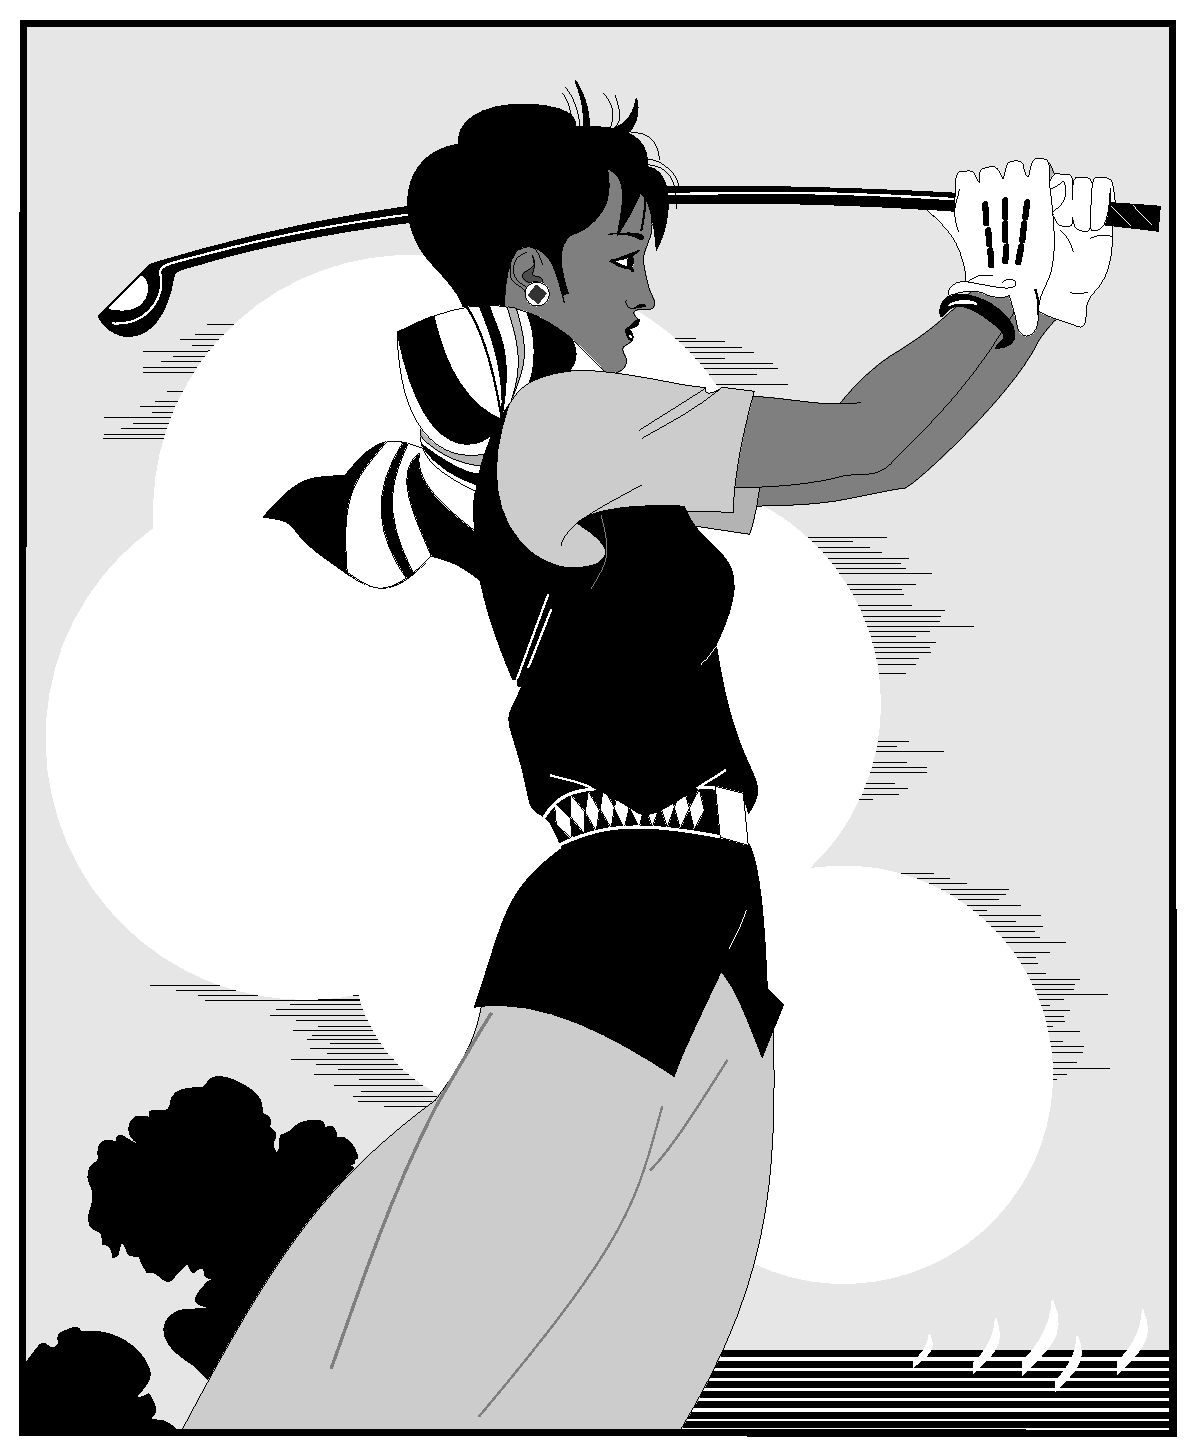
\includegraphics[width = 0.4\textwidth]{golfer}
\bicaption[golfer1]{}{打高尔夫球球的人(博士论文双语题注)}{Fig.$\!$}{The person playing golf (Doctoral thesis)}
\end{figure}

每个图均应有图题(由图序和图名组成),图题不宜有标点符号,图名在图序之后空1个半
角字符排写。图序按章编排,如第1章第一个插图的图号为“图1-1”。图题置于图下,硕士论
文只用中文,博士论文用中、英两种文字,居中书写,中文在上,要求中文用宋体5号字,
英文用Times New Roman 5号字。有图注或其它说明时应置于图题之上。引用图应注明出处
,在图题右上角加引用文献号。图中若有分图时,分图题置于分图之下或图题之下,可以只
用中文书写,分图号用a)、b)等表示。图中各部分说明应采用中文(引用的外文图除外)或
数字符号,各项文字说明置于图题之上(有分图时,置于分图题之上)。图中文字用宋体、
Times New Roman字体,字号尽量采用5号字(当字数较多时可用小5号字,以清晰表达为原
则,但在一个插图内字号要统一)。同一图内使用文字应统一。图表中物理量、符号用斜体
。
\subsection{本硕论文题注}[Other picture example]

本硕论文题注如\figref{fig:bm}所示。

\begin{figure}[ht]
\centering
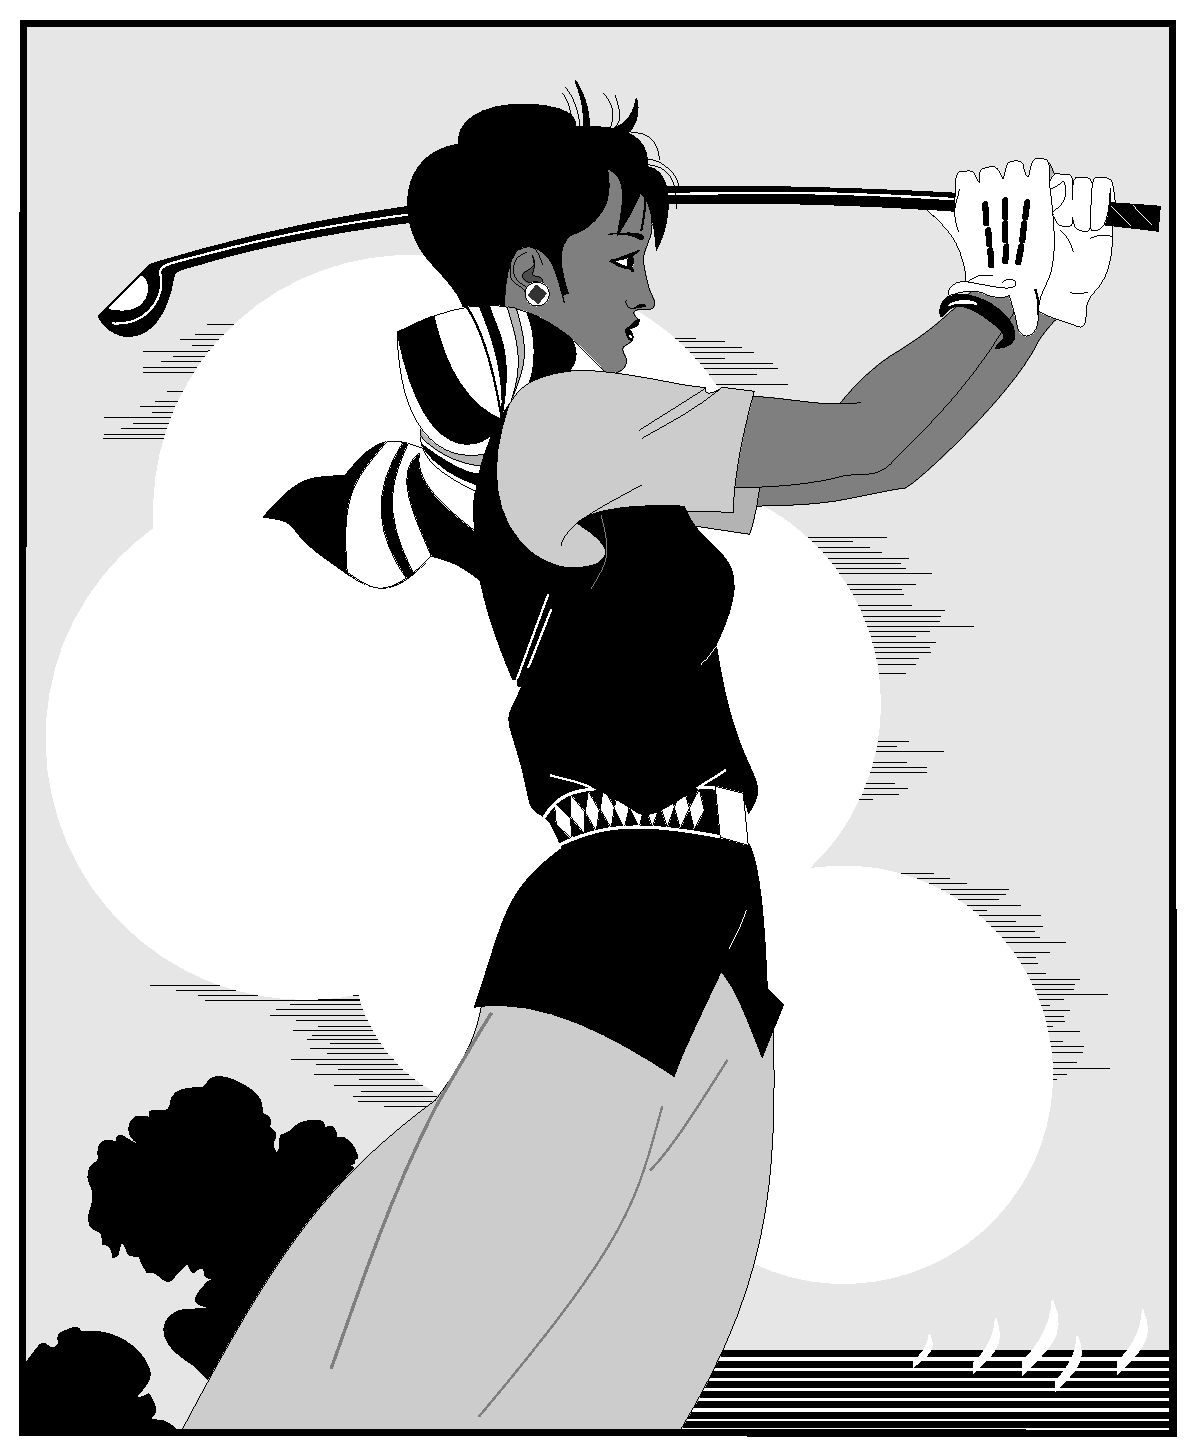
\includegraphics[width = 0.4\textwidth]{golfer}
\caption{打高尔夫球的人,硕士论文要求只用汉语}
\label{fig:bm}
\end{figure}

\subsection{并排图和子图}[Abreast-picture and Sub-picture example]
\subsubsection{并排图}[Abreast-picture example]

使用并排图时,需要注意对齐方式。默认情况是中部对齐。这里给出中部对齐、顶部对齐
、图片底部对齐三种常见方式。其中,底部对齐方式有一个很巧妙的方式,将长度比较小
的图放在左面即可。

\lipsum[2]

\begin{figure}[htbp]
\centering
\begin{minipage}{0.4\textwidth}
\centering
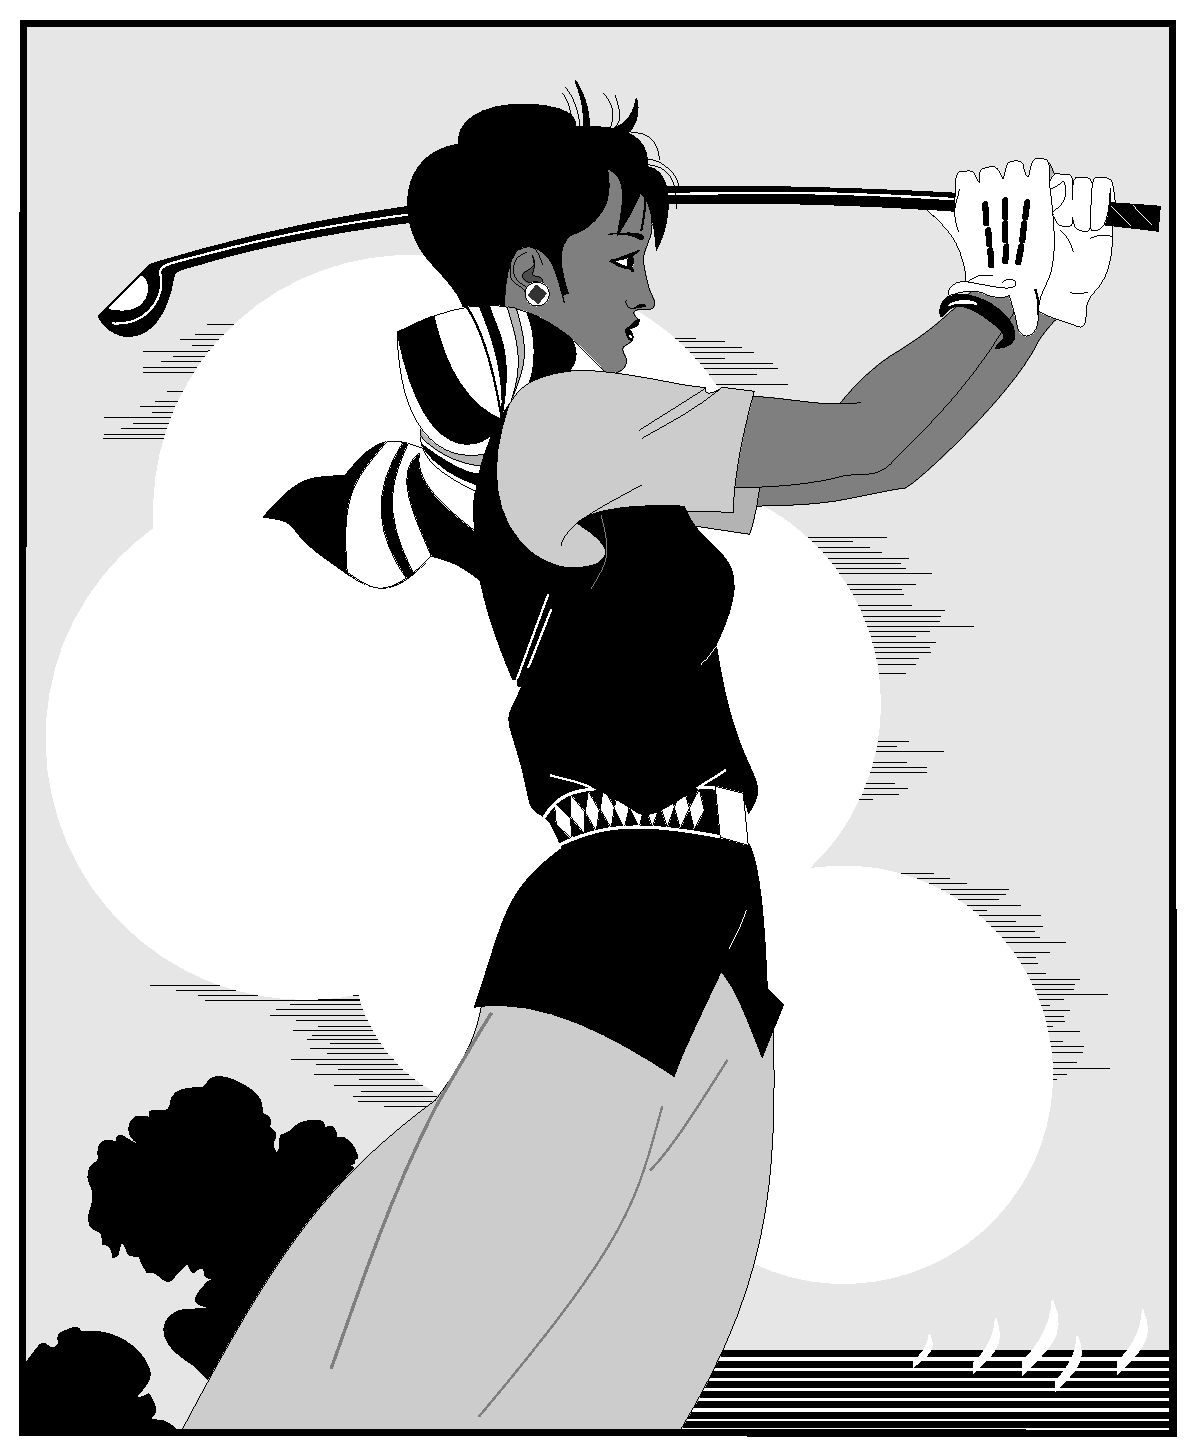
\includegraphics[width=\textwidth]{golfer}
\bicaption[golfer2]{}{打高尔夫球的人}{Fig.$\!$}{The person playing golf}
\end{minipage}
\centering
\begin{minipage}{0.4\textwidth}
\centering
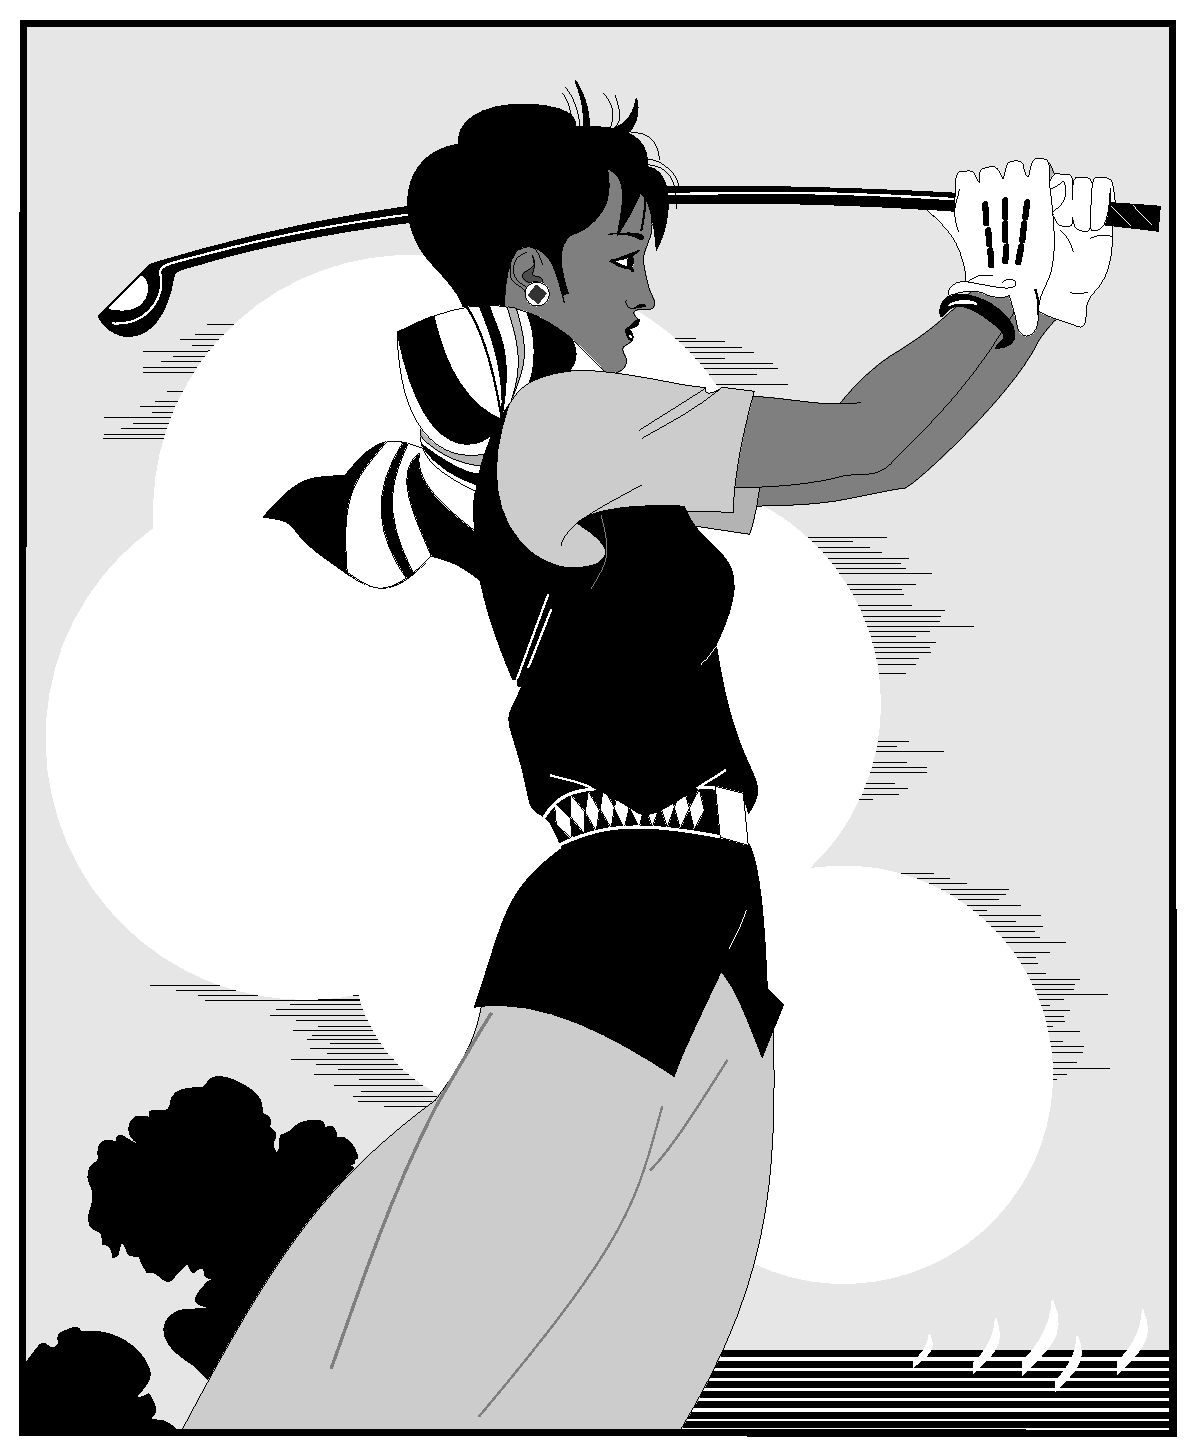
\includegraphics[width=\textwidth]{golfer}
\bicaption[golfer3]{}{打高尔夫球的人。注意,这里默认居中}{Fig.$\!$}{The person playing golf. Please note that, it is vertically center aligned by default.}
\end{minipage}
\end{figure}

\begin{figure}[htbp]
\centering
\begin{minipage}[t]{0.4\textwidth}
\centering
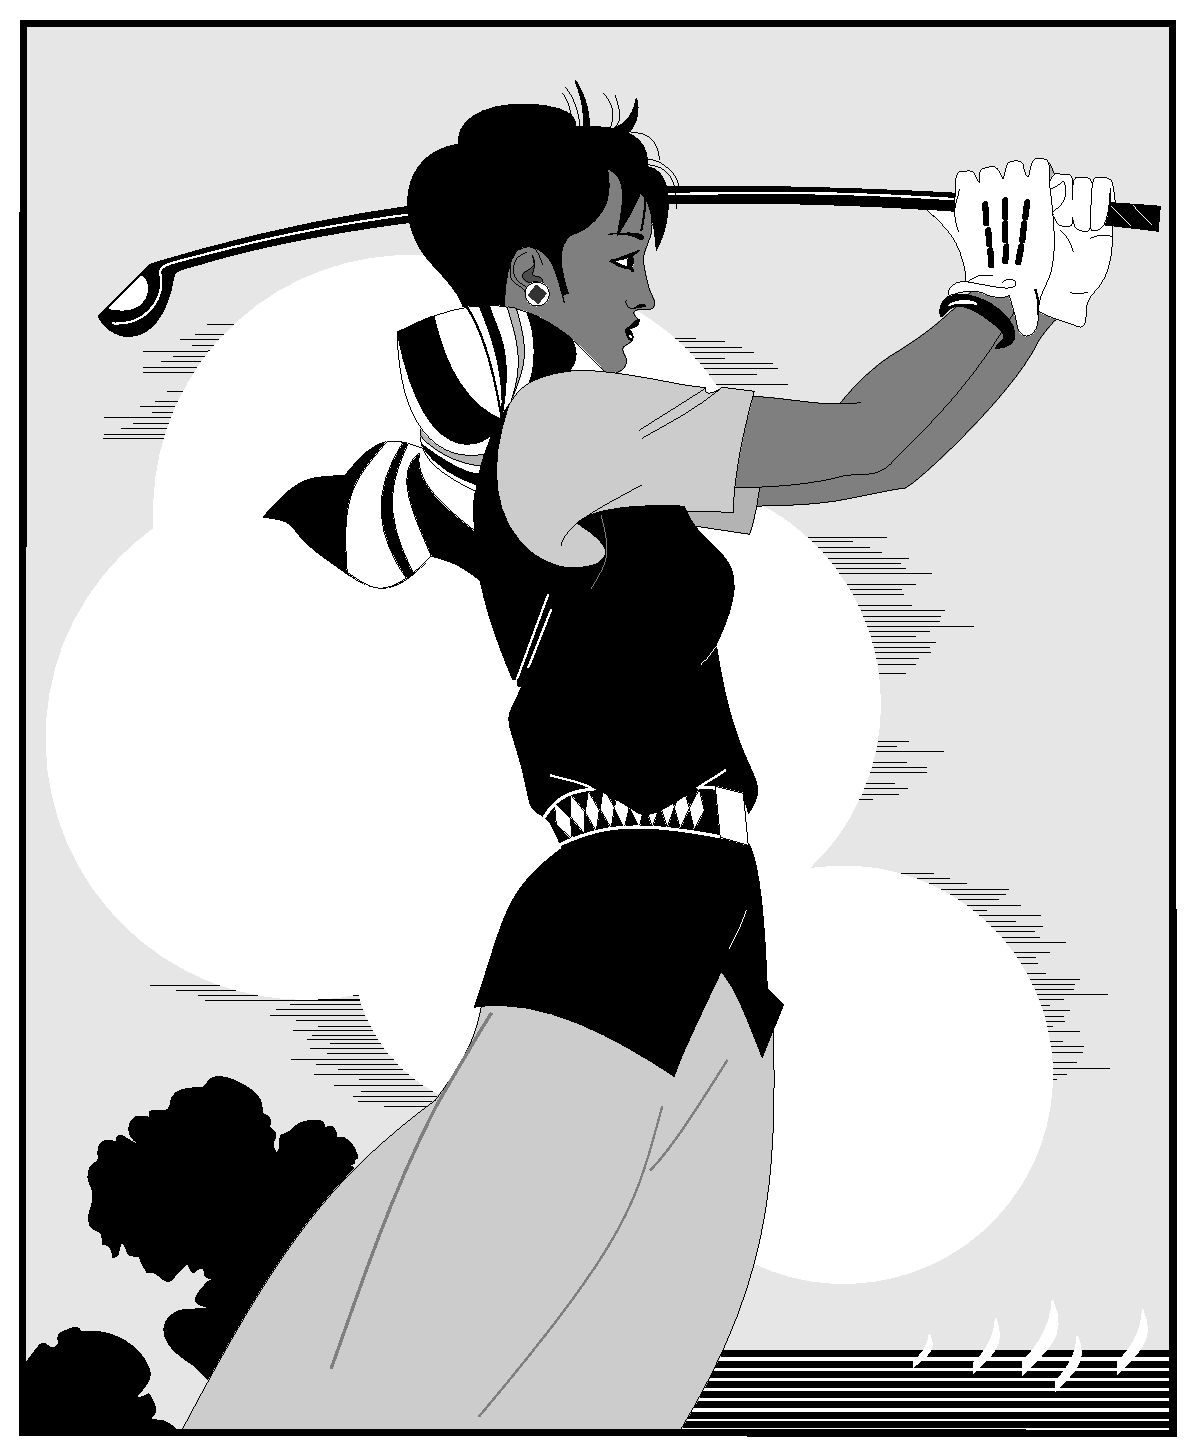
\includegraphics[width=\textwidth]{golfer}
\bicaption[golfer5]{}{打高尔夫球的人}{Fig.$\!$}{The person playing golf}
\end{minipage}
\centering
\begin{minipage}[t]{0.4\textwidth}
\centering
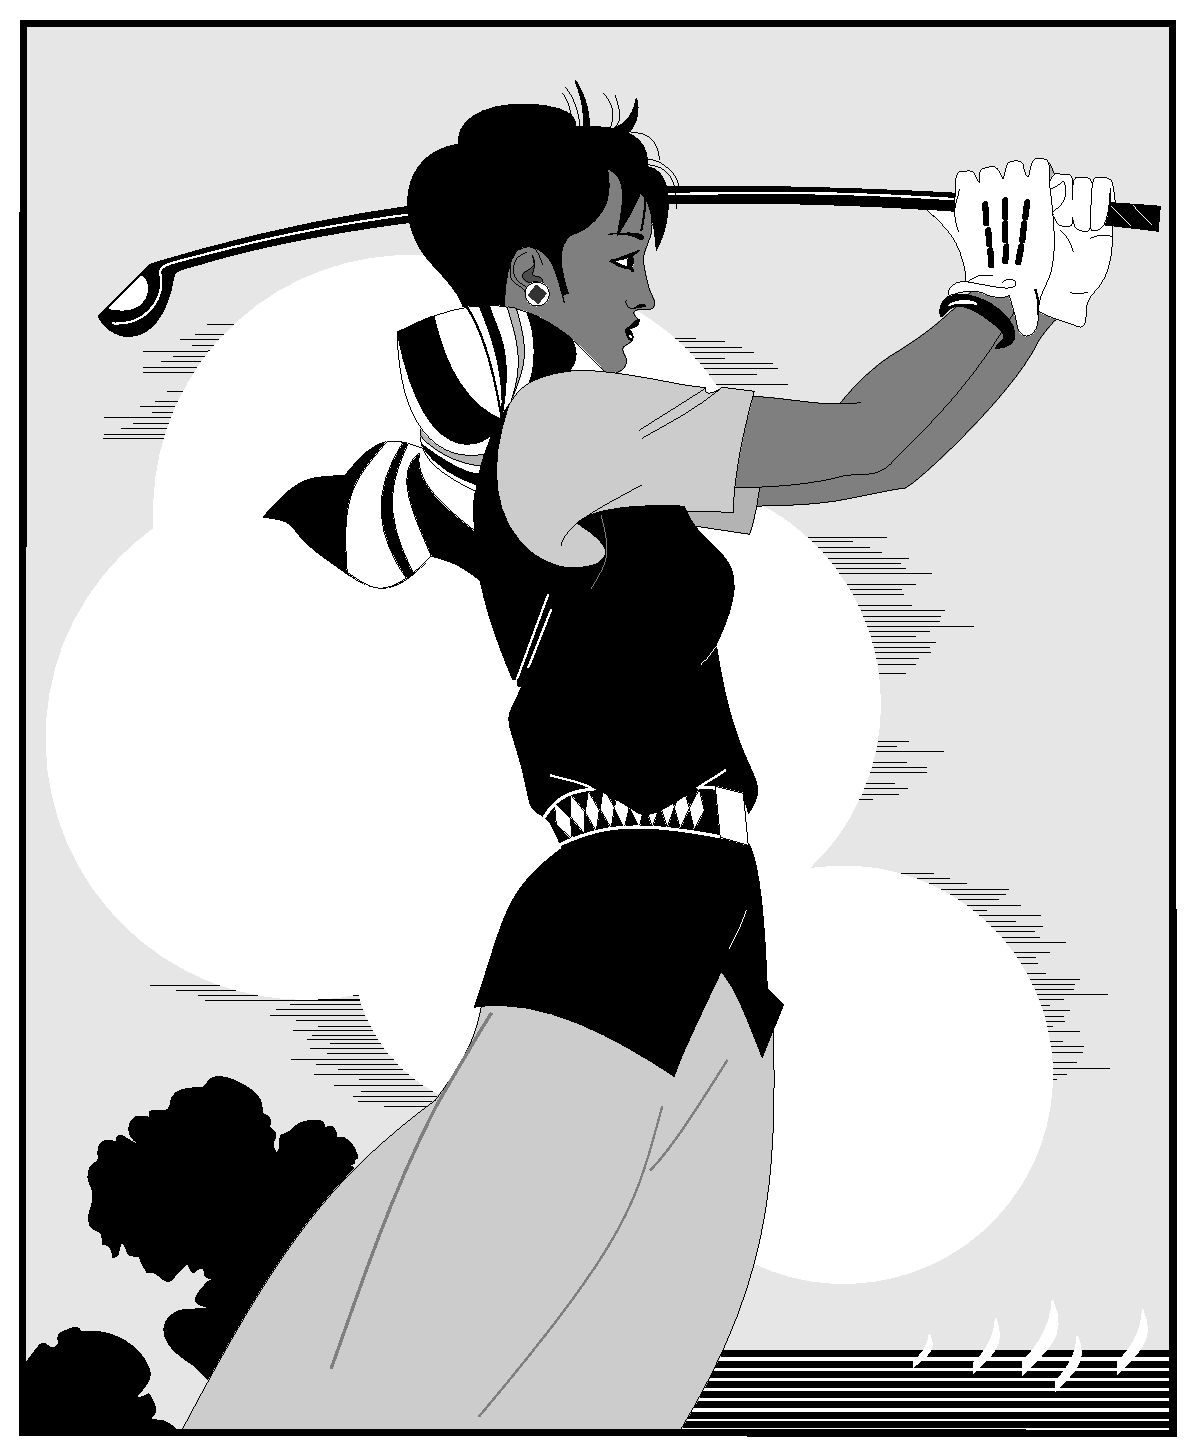
\includegraphics[width=\textwidth]{golfer}
\bicaption[golfer8]{}{打高尔夫球的人。注意,此图是顶部对齐}{Fig.$\!$}{The person playing golf. Please note that, it is vertically top aligned.}
\end{minipage}
\end{figure}

\begin{figure}[htbp]
\centering
\begin{minipage}[t]{0.4\textwidth}
\centering
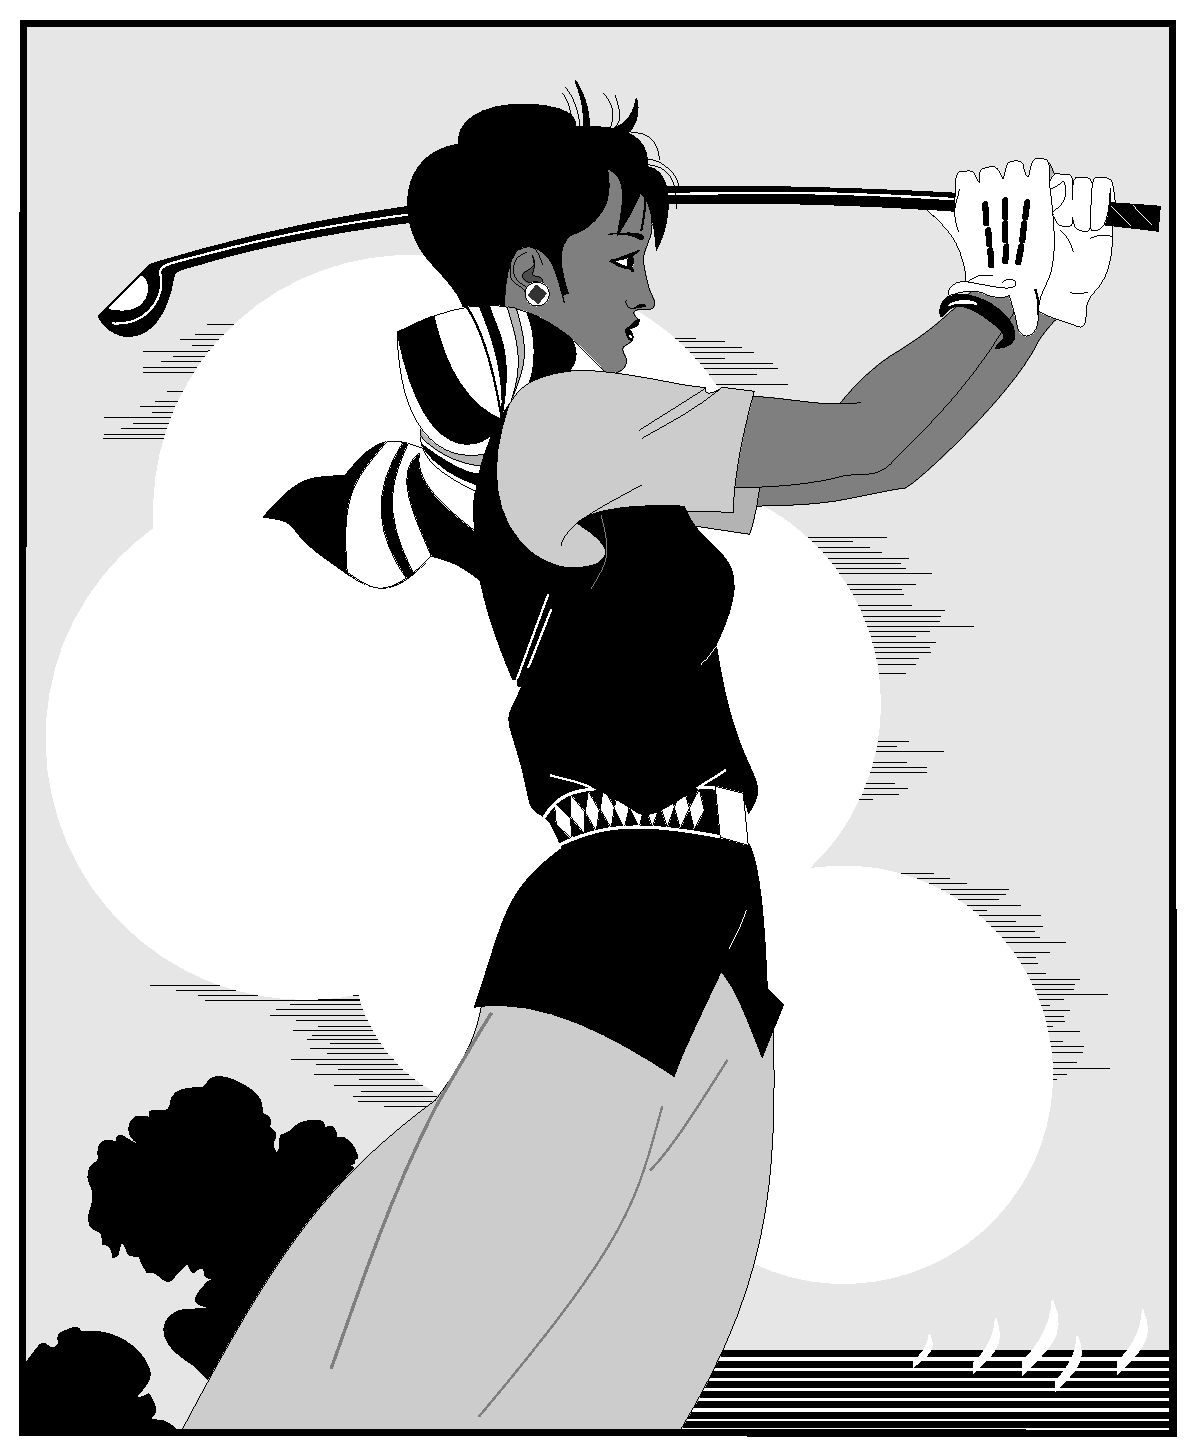
\includegraphics[width=\textwidth,height=\textwidth]{golfer}
\bicaption[golfer9]{}{打高尔夫球的人。注意,此图对齐方式是图片底部对齐}{Fig.$\!$}{The person playing golf. Please note that, it is vertically bottom aligned for figure.}
\end{minipage}
\centering
\begin{minipage}[t]{0.4\textwidth}
\centering
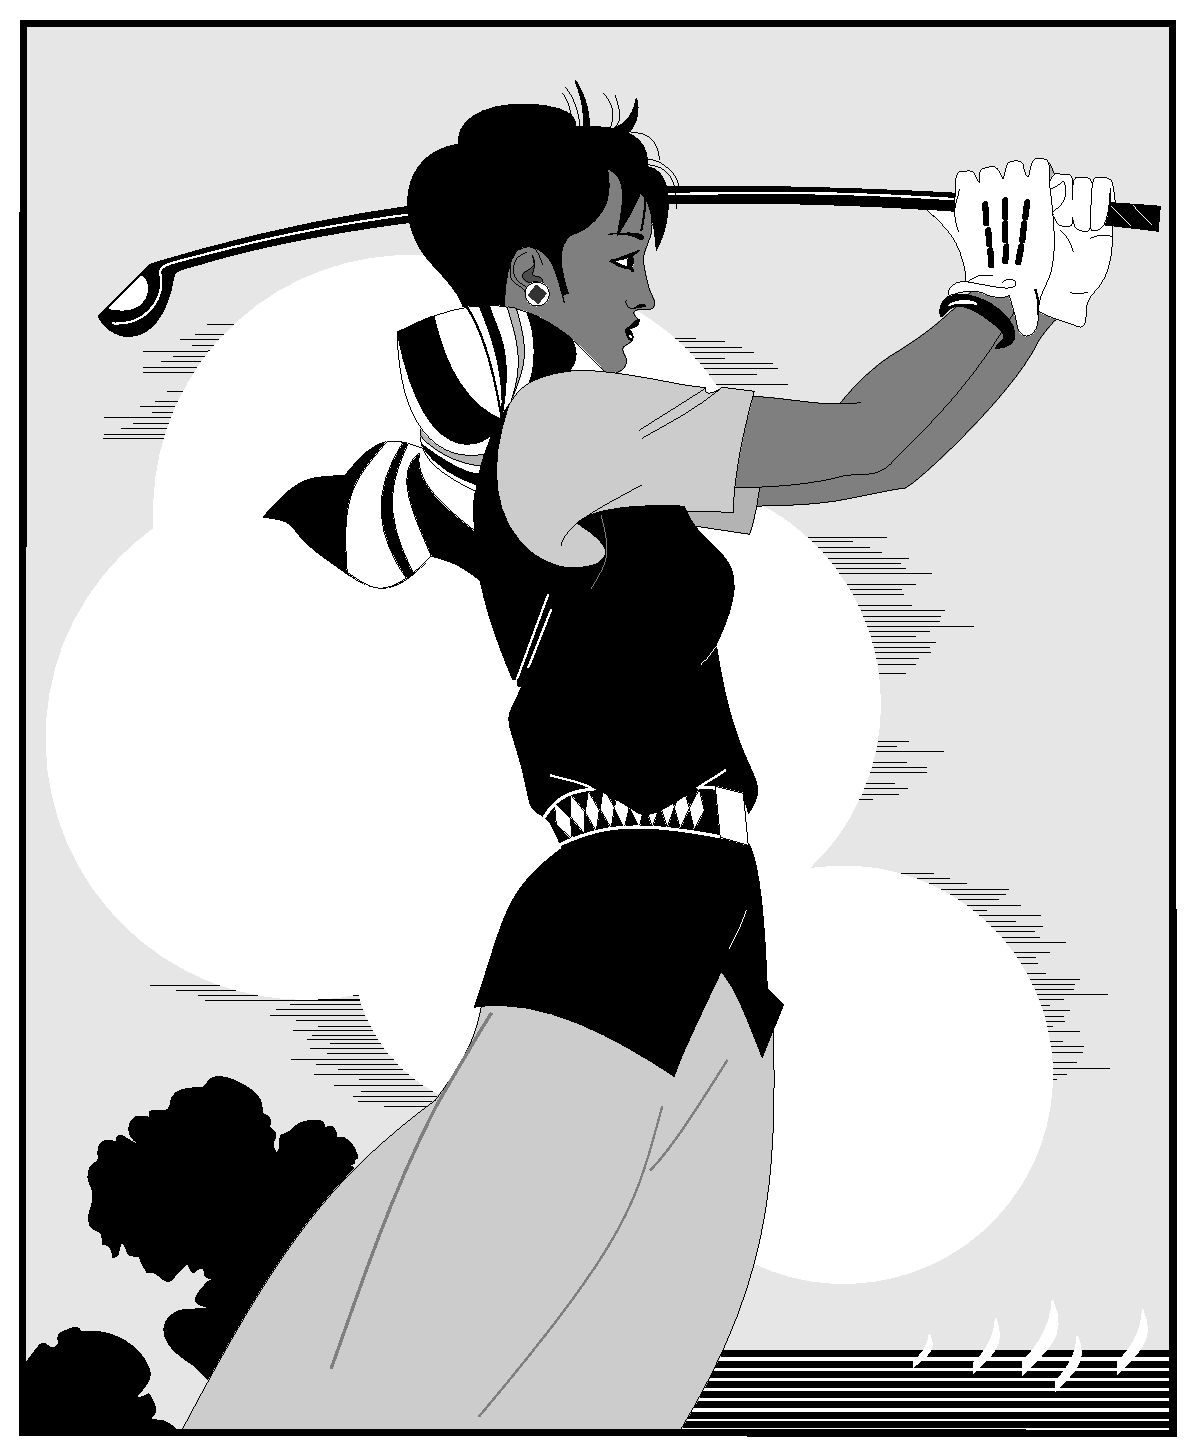
\includegraphics[width=\textwidth]{golfer}
\bicaption[golfer6]{}{打高尔夫球的人}{Fig.$\!$}{The person playing golf}
\end{minipage}
\end{figure}

\subsubsection{子图}[Sub-picture example]

注意:子图题注也可以只用中文。规范规定“分图题置于分图之下或图题之下”,但没有给出具体的格式要求。
没有要求的另外一个说法就是“无论什么格式都不对”。
所以只有在一个图中有标注“a),b)”,无法使用\cs{subfigure}的情况下,使用最后一个图例中的格式设置方法,否则不要使用。
为了应对“无论什么格式都不对”,这个子图图题使用“minipage”和“description”环境,宽度,对齐方式可以按照个人喜好自由设置,是否使用双语子图图题也可以自由设置。

\lipsum[1-3]

无意义文字,每页底部不要留空白。

\lipsum[1]

\begin{figure}[!ht]
\setlength{\subfigcapskip}{-1bp}
\centering
\begin{minipage}{\textwidth}
\centering
\subfigure{\label{golfer41}}\addtocounter{subfigure}{-2}
\subfigure[The person playing golf]{\subfigure[打高尔夫球的人~1]{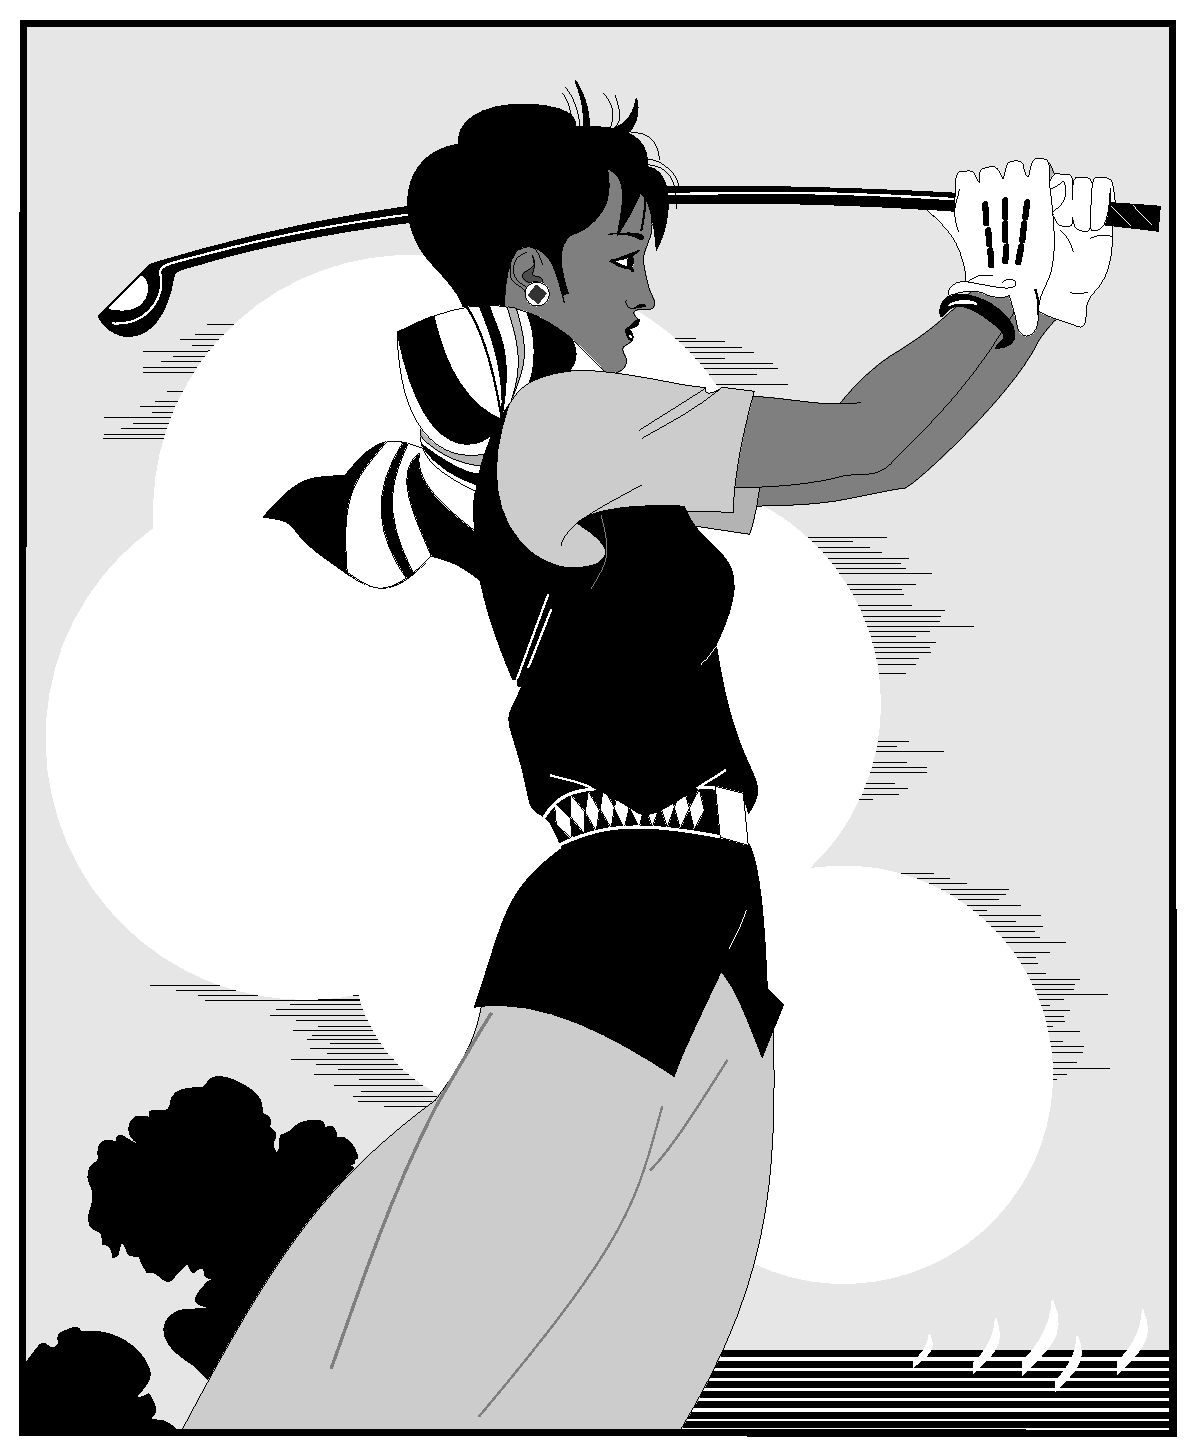
\includegraphics[width=0.4\textwidth]{golfer}}}
\hspace{2em}
\subfigure{\label{golfer42}}\addtocounter{subfigure}{-2}
\subfigure[The person playing golf]{\subfigure[打高尔夫球的人~2]{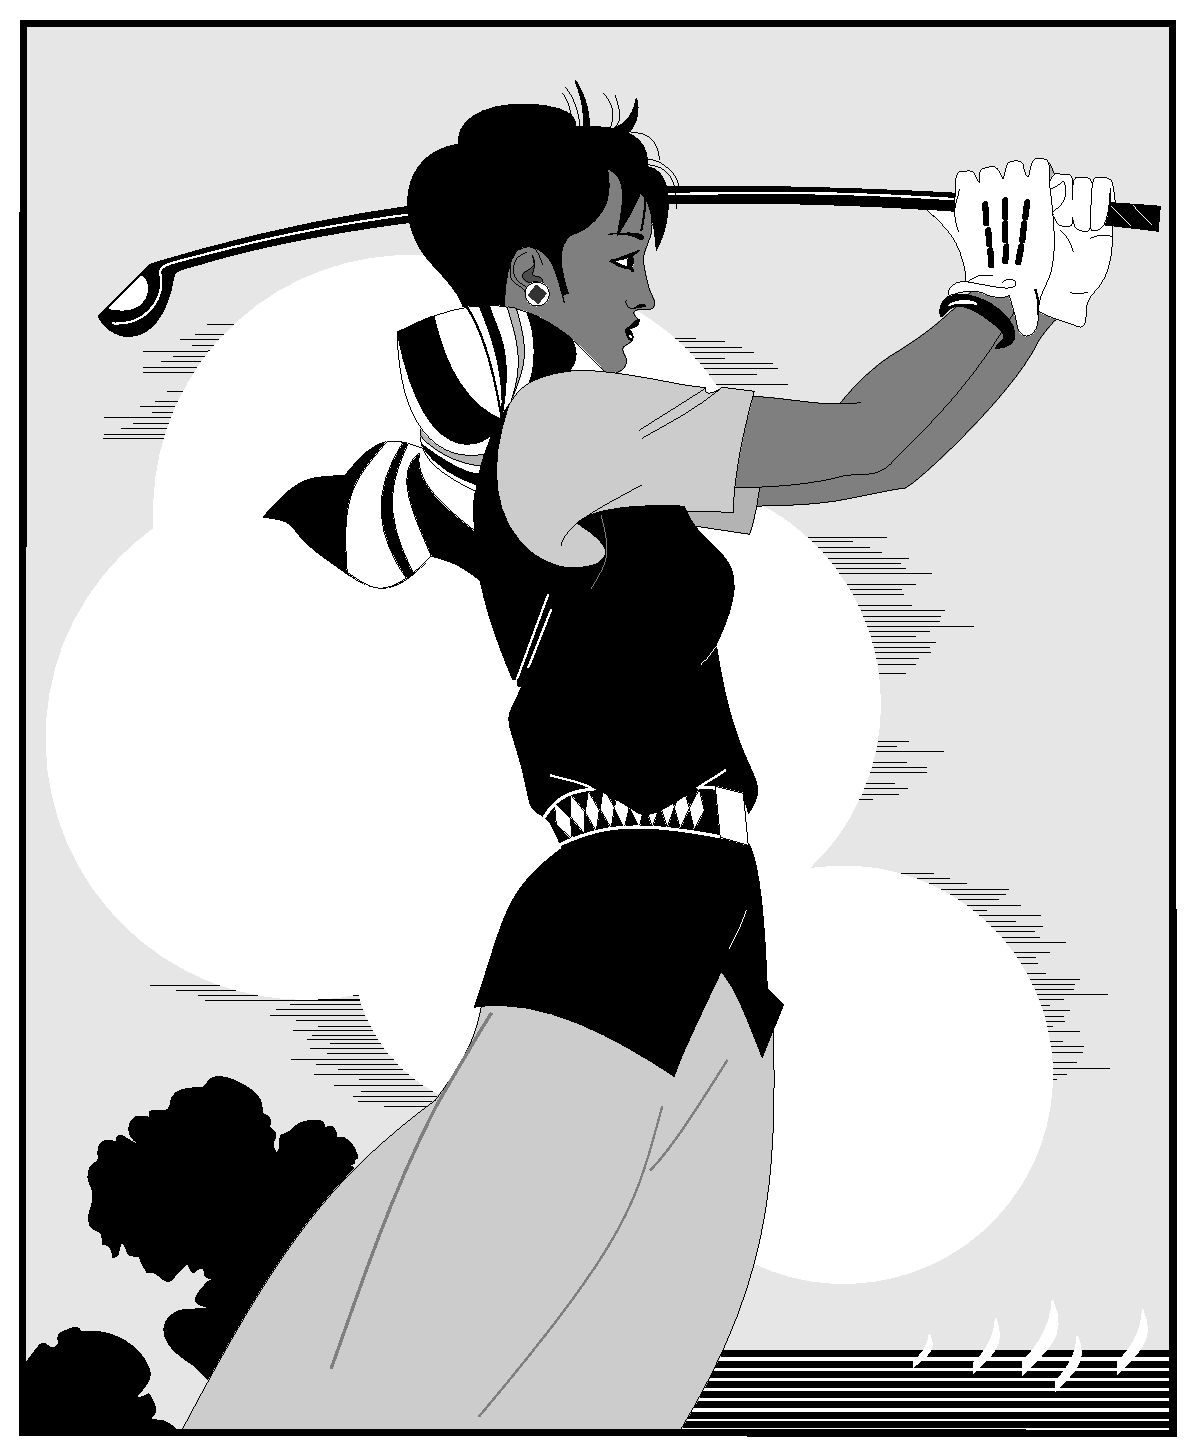
\includegraphics[width=0.4\textwidth]{golfer}}}
\end{minipage}
\centering
\begin{minipage}{\textwidth}
\centering
\subfigure{\label{golfer43}}\addtocounter{subfigure}{-2}
\subfigure[The person playing golf]{\subfigure[打高尔夫球的人~3]{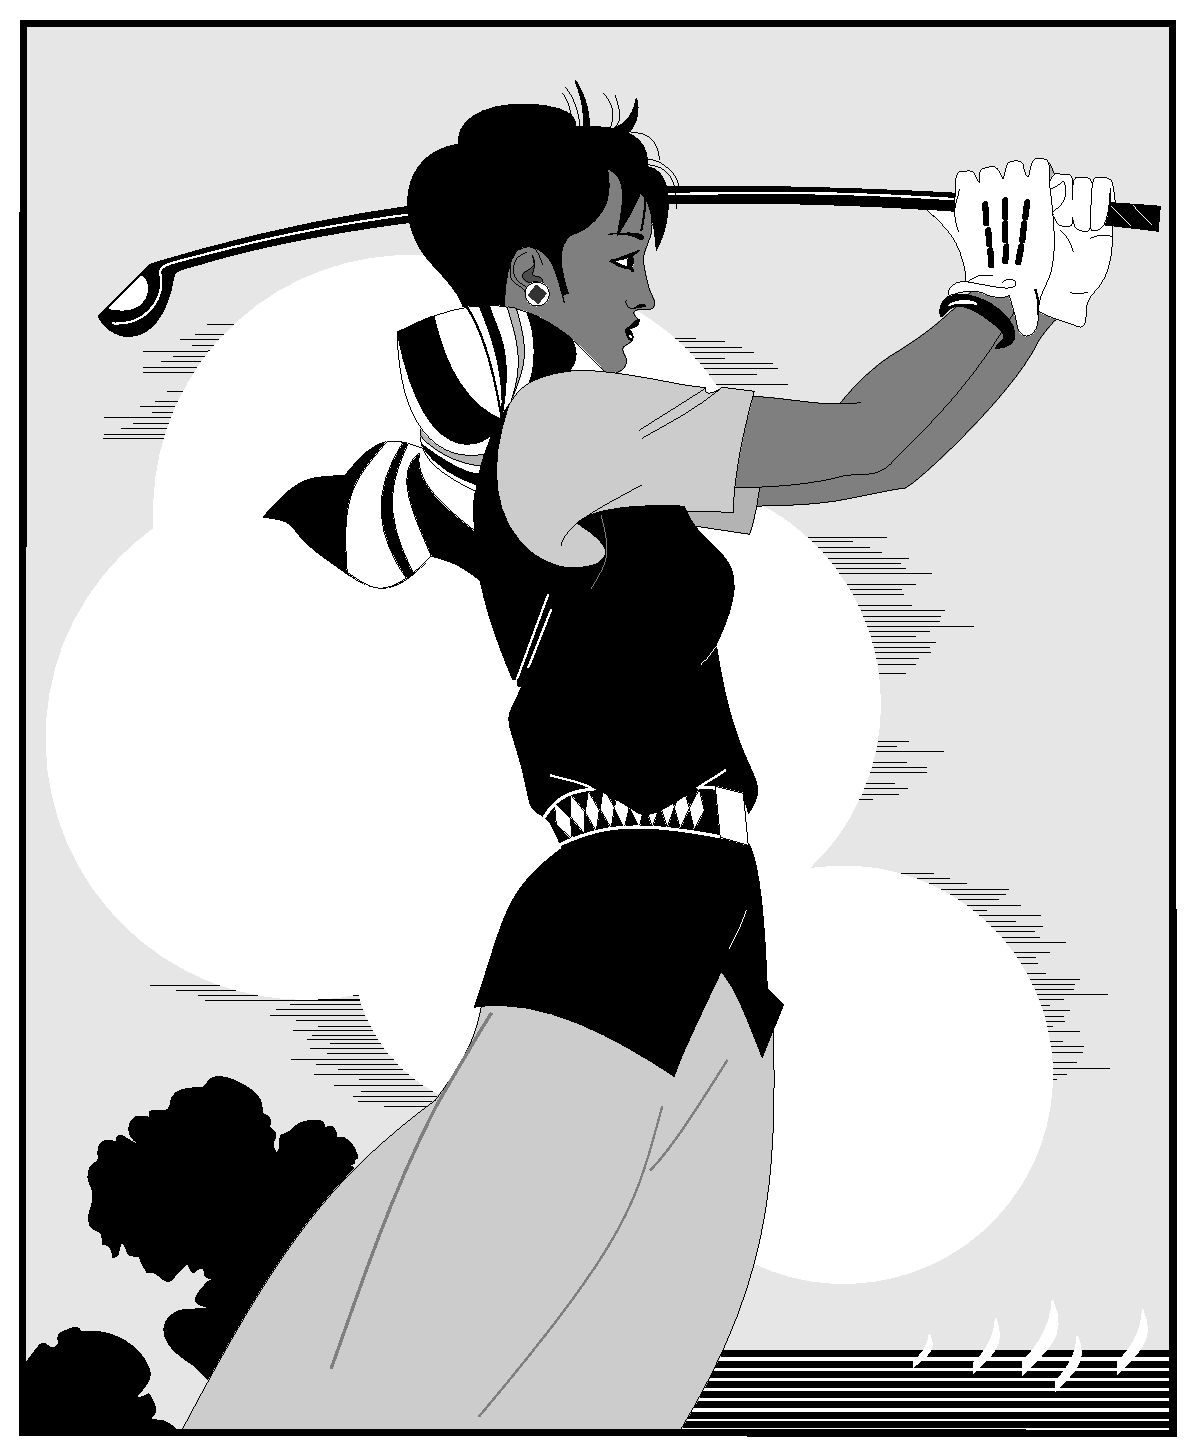
\includegraphics[width=0.4\textwidth]{golfer}}}
\hspace{2em}
\subfigure{\label{golfer44}}\addtocounter{subfigure}{-2}
\subfigure[The person playing golf. Here, 'hang indent' and 'center last line' are not stipulated in the regulation.]{\subfigure[打高尔夫球的人~4。注意,规范中没有明确规定要悬挂缩进、最后一行居中。]{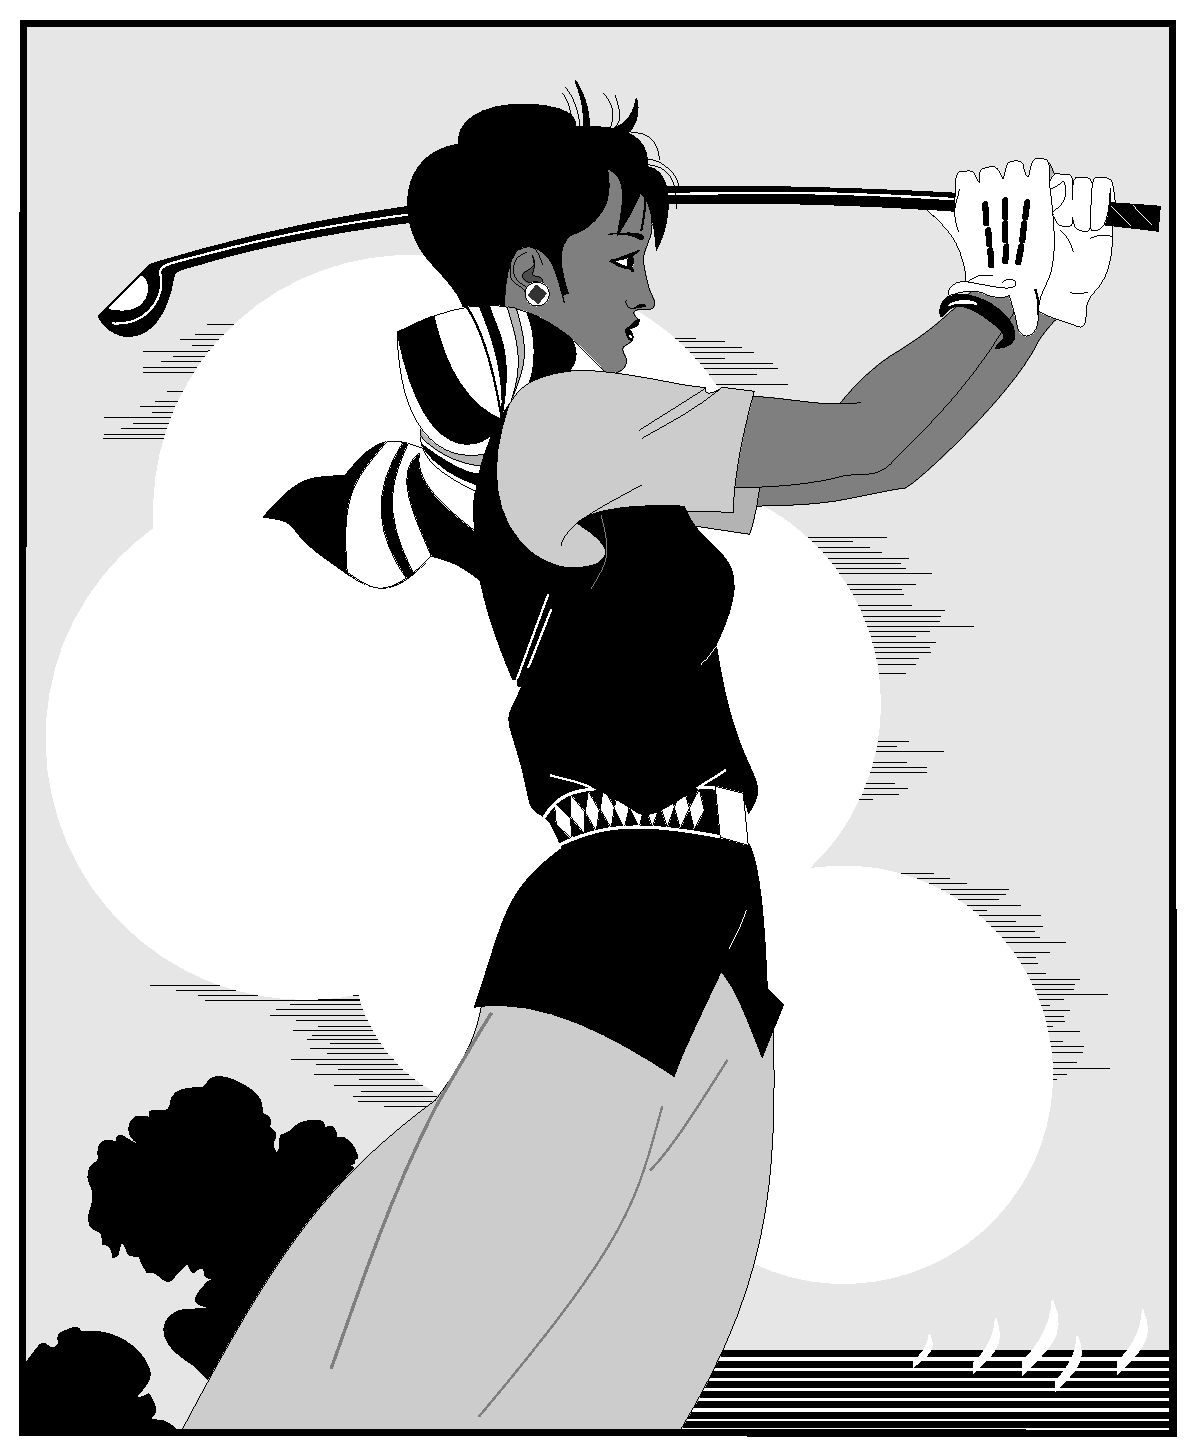
\includegraphics[width=0.4\textwidth]{golfer}}}
\end{minipage}
\vspace{0.2em}
\bicaption[golfer4]{}{打高尔夫球的人}{Fig.$\!$}{The person playing gol}
\end{figure}

\begin{figure}[t]
  \centering
  \begin{minipage}{.7\linewidth}
    \setlength{\subfigcapskip}{-1bp}
    \centering
    \begin{minipage}{\textwidth}
      \centering
      \subfigure{\label{golfer45}}\addtocounter{subfigure}{-2}
      \subfigure[The person playing golf]{\subfigure[打高尔夫球的人~1]{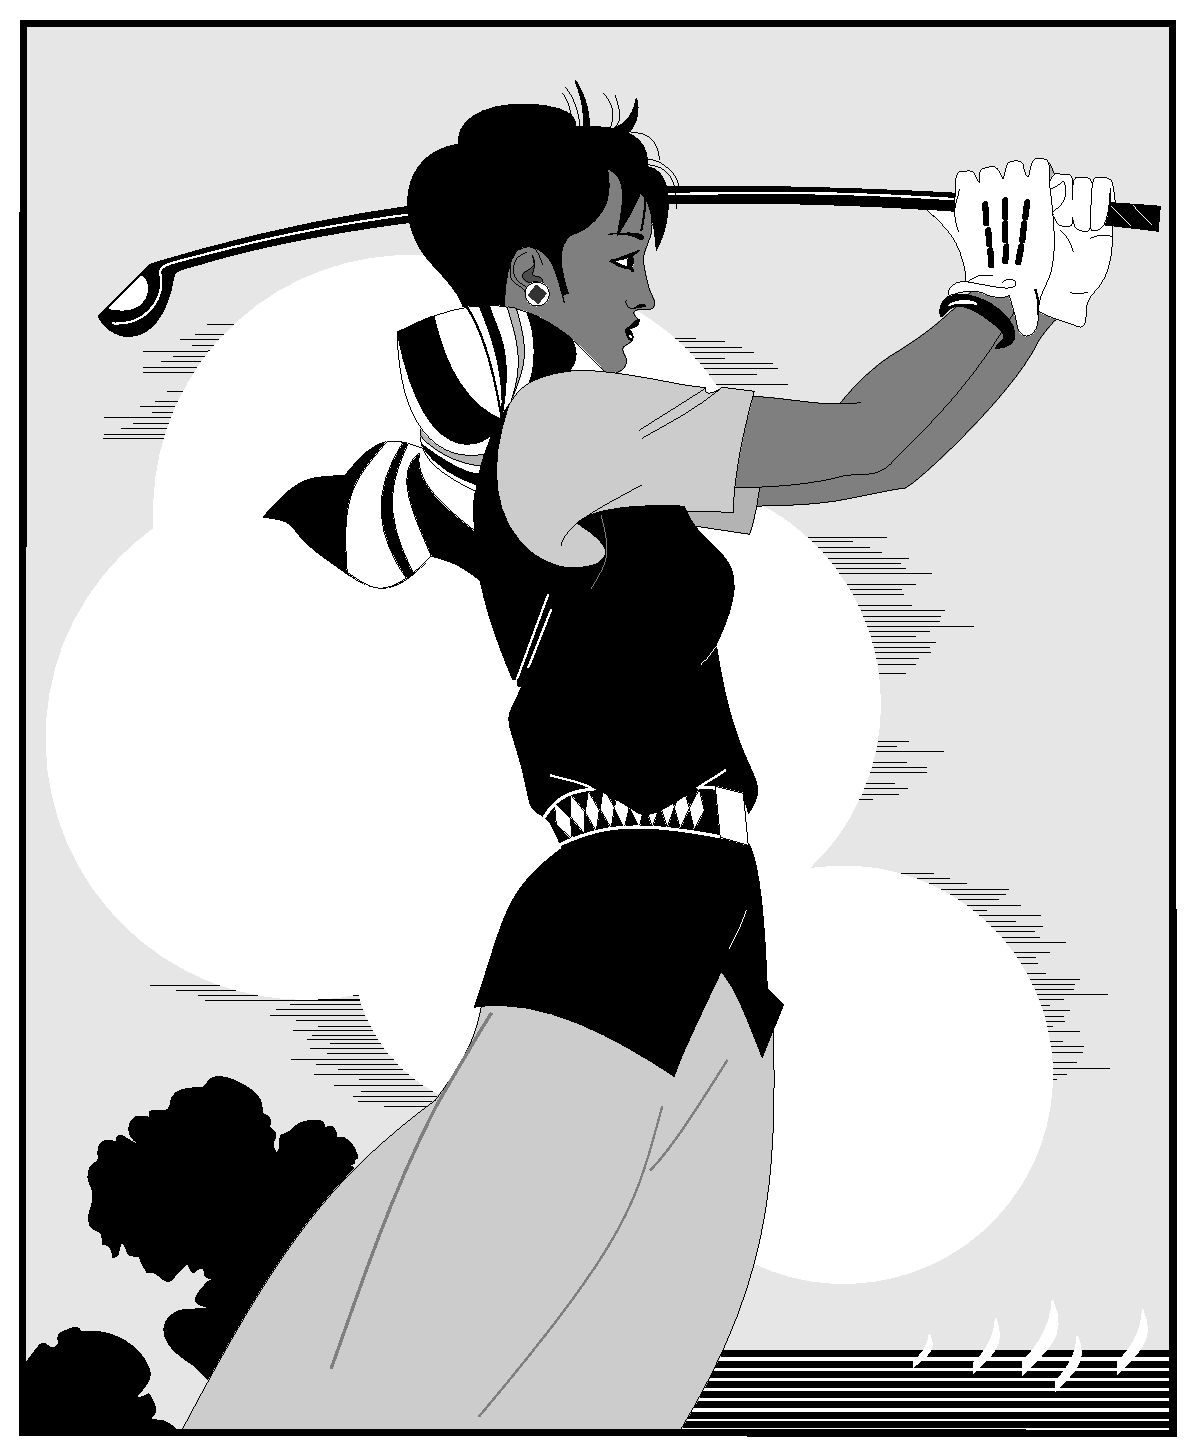
\includegraphics[width=0.4\textwidth]{golfer}}}
      \hspace{4em}
      \subfigure{\label{golfer46}}\addtocounter{subfigure}{-2}
      \subfigure[The person playing golf]{\subfigure[打高尔夫球的人~2]{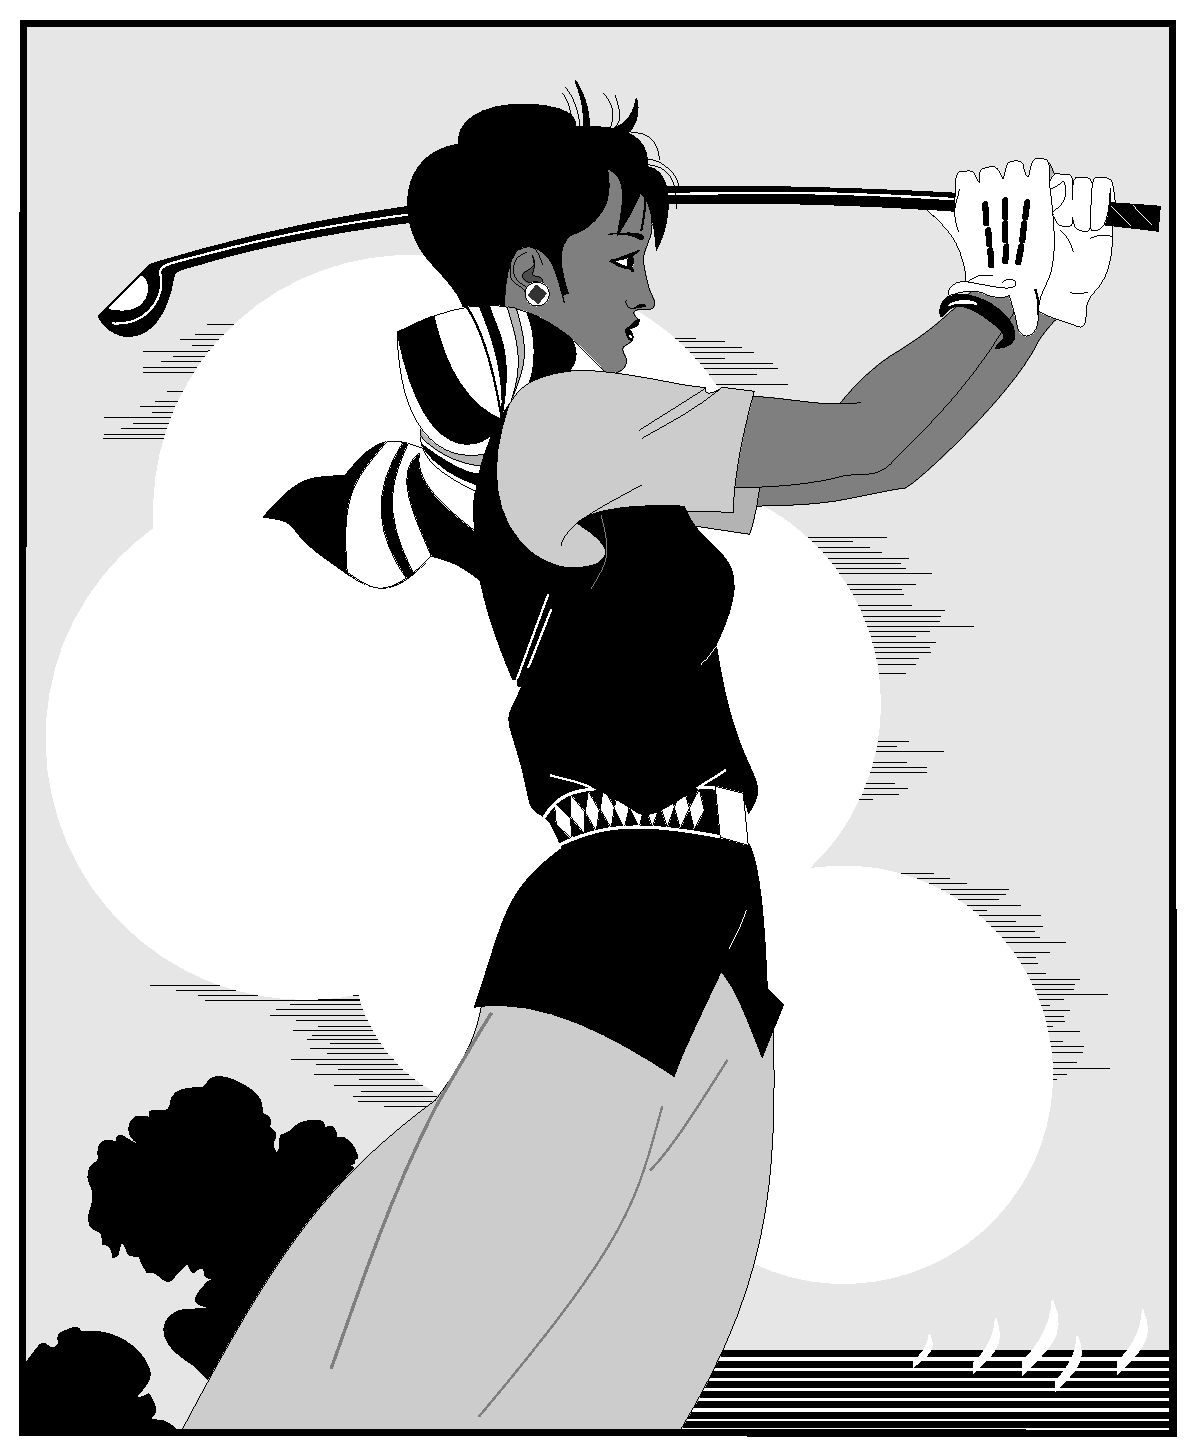
\includegraphics[width=0.4\textwidth]{golfer}}}
    \end{minipage}
    \vskip 0.2em
  \wuhao 注意:这里是中文图注添加位置(我工要求,图注在图题之上)。
    \vspace{0.2em}
\bicaption[golfer47]{}{打高尔夫球的人。注意,此处我工有另外一处要求,子图图题可以位于主图题之下。但由于没有明确说明位于下方具体是什么格式,所以这里不给出举例。}{Fig.$\!$}{The person playing golf. Please note that, although it is appropriate to put subfigures' captions under this caption as stipulated in regulation, but its format is not clearly stated.}
  \end{minipage}
\end{figure}

\begin{figure}[t]
\centering
\begin{tikzpicture}
	\node[anchor=south west,inner sep=0] (image) at (0,0) {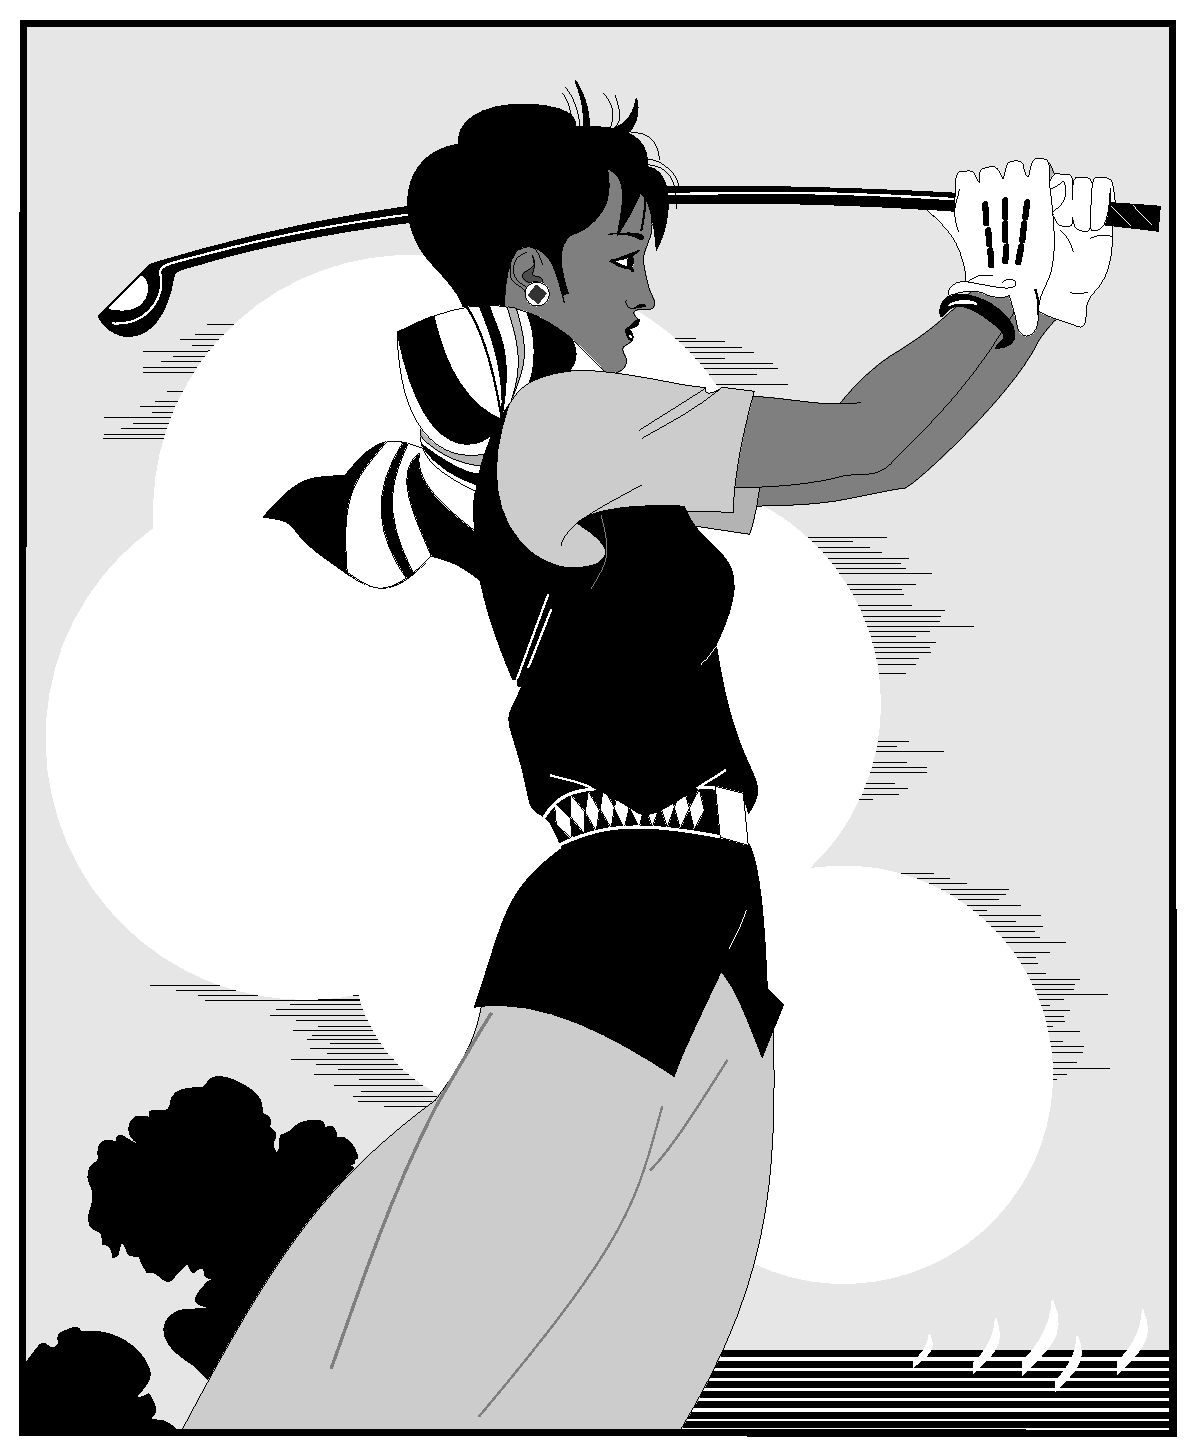
\includegraphics[width=0.3\textwidth]{golfer}};
	\begin{scope}[x={(image.south east)},y={(image.north west)}]
		\node at (0.3,0.5) {a)};
		\node at (0.8,0.2) {b)};
	\end{scope}
\end{tikzpicture}
\bicaption[golfer0]{}{打高尔夫球球的人(博士论文双语题注)}{Fig.$\!$}{The person playing golf (Doctoral thesis)}
\vskip -0.4em
 \hspace{2em}
\begin{minipage}[t]{0.3\textwidth}
\wuhao \setlist[description]{font=\normalfont}
	\begin{description}
		\item[a)]子图图题
	\end{description}
 \end{minipage}
 \hspace{2em}
 \begin{minipage}[t]{0.3\textwidth}
\wuhao \setlist[description]{font=\normalfont}
	\begin{description}
		\item[b)]子图图题
		\item[b)]Subfigure caption
	\end{description}
\end{minipage}
\end{figure}


\begin{figure}[!ht]
	\centering
	\begin{sideways}
		\begin{minipage}{\textheight}
			\centering
			\fbox{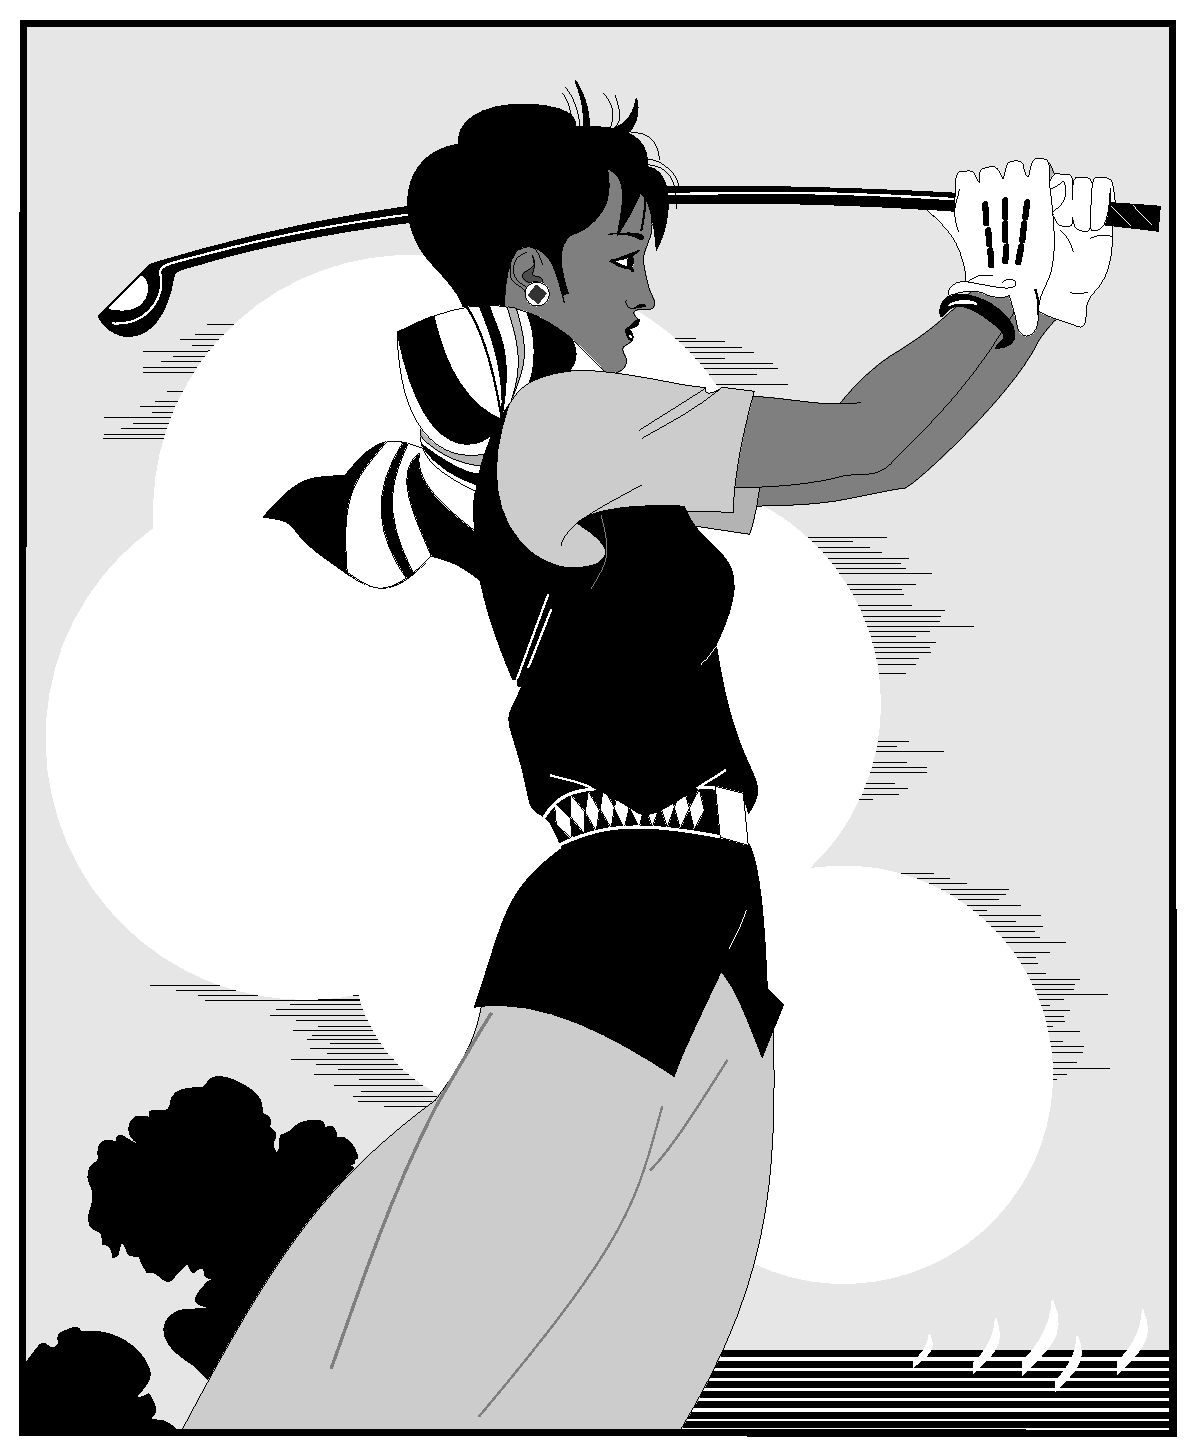
\includegraphics[width=0.2\textwidth]{golfer}}
			\fbox{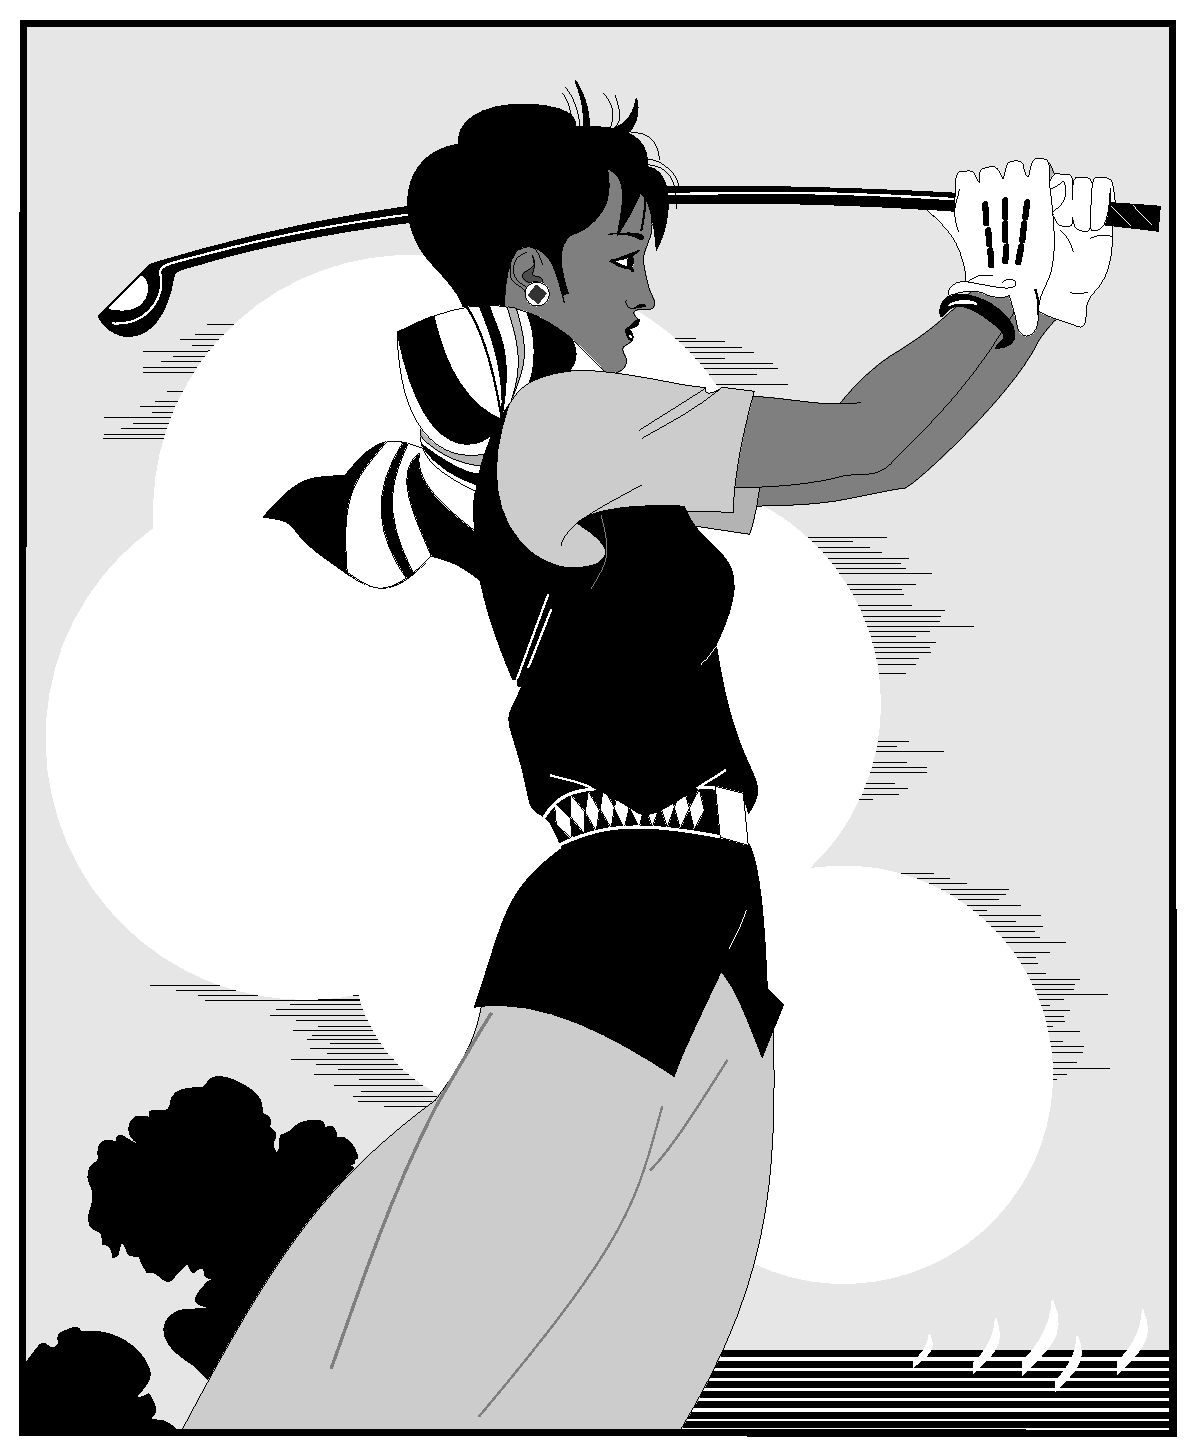
\includegraphics[width=0.2\textwidth]{golfer}}
			\fbox{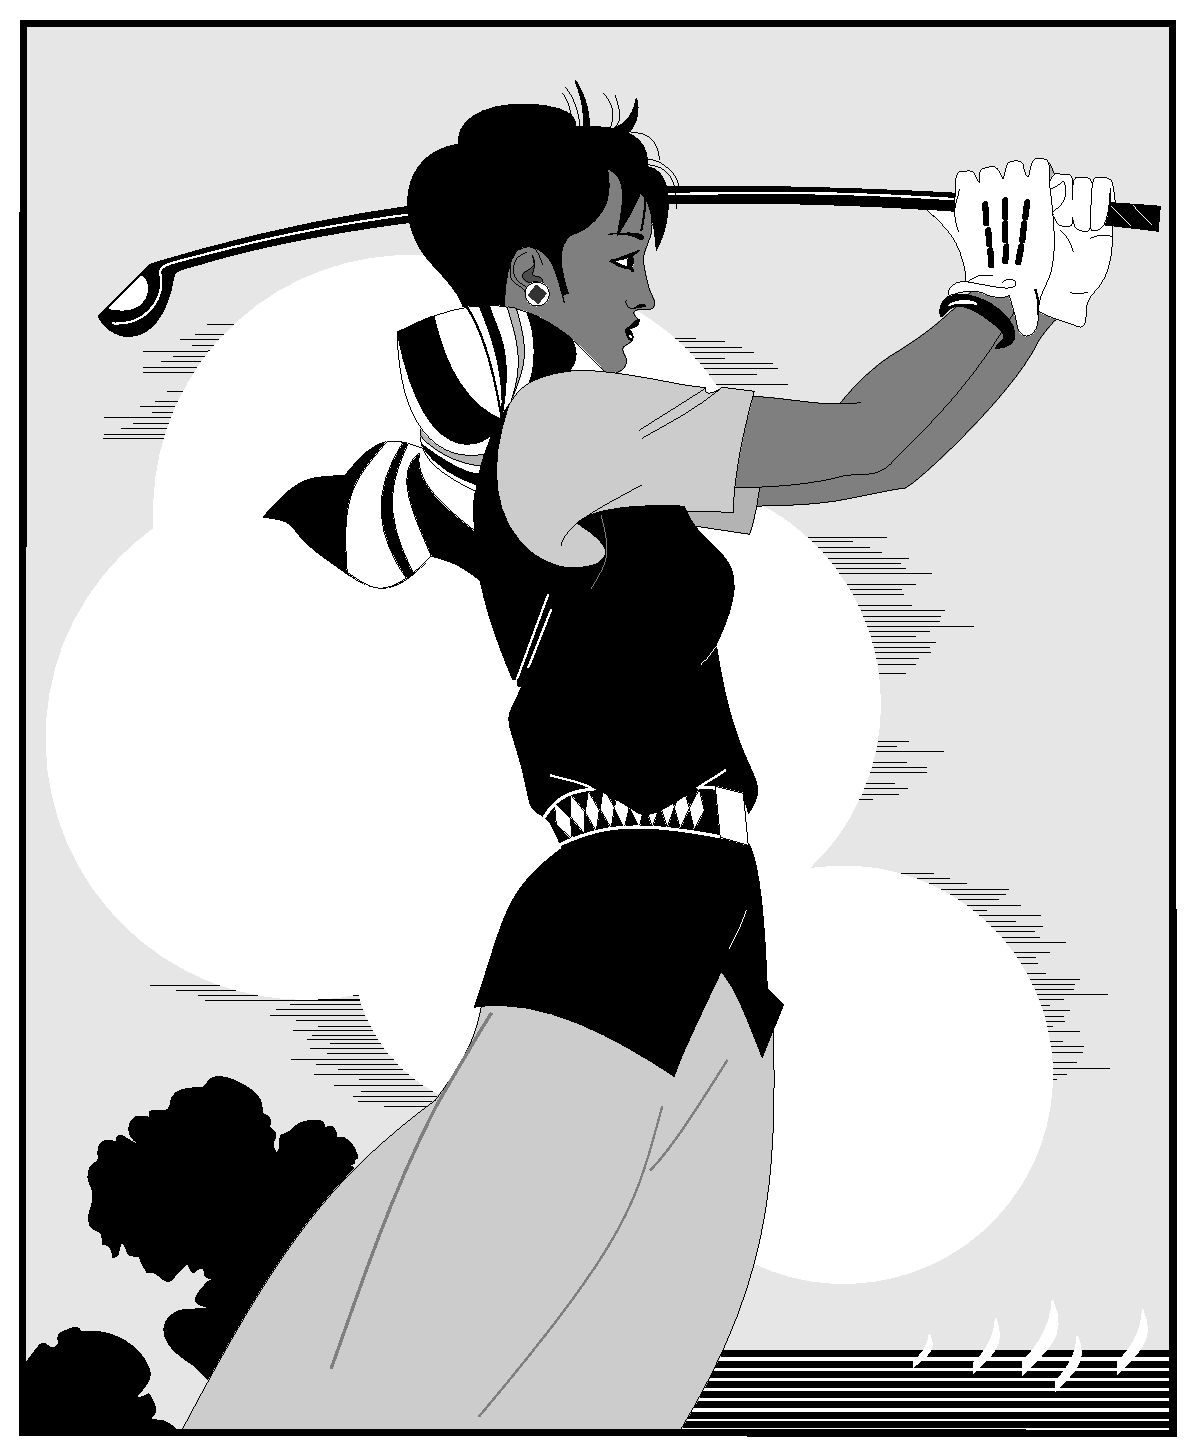
\includegraphics[width=0.2\textwidth]{golfer}}
			\fbox{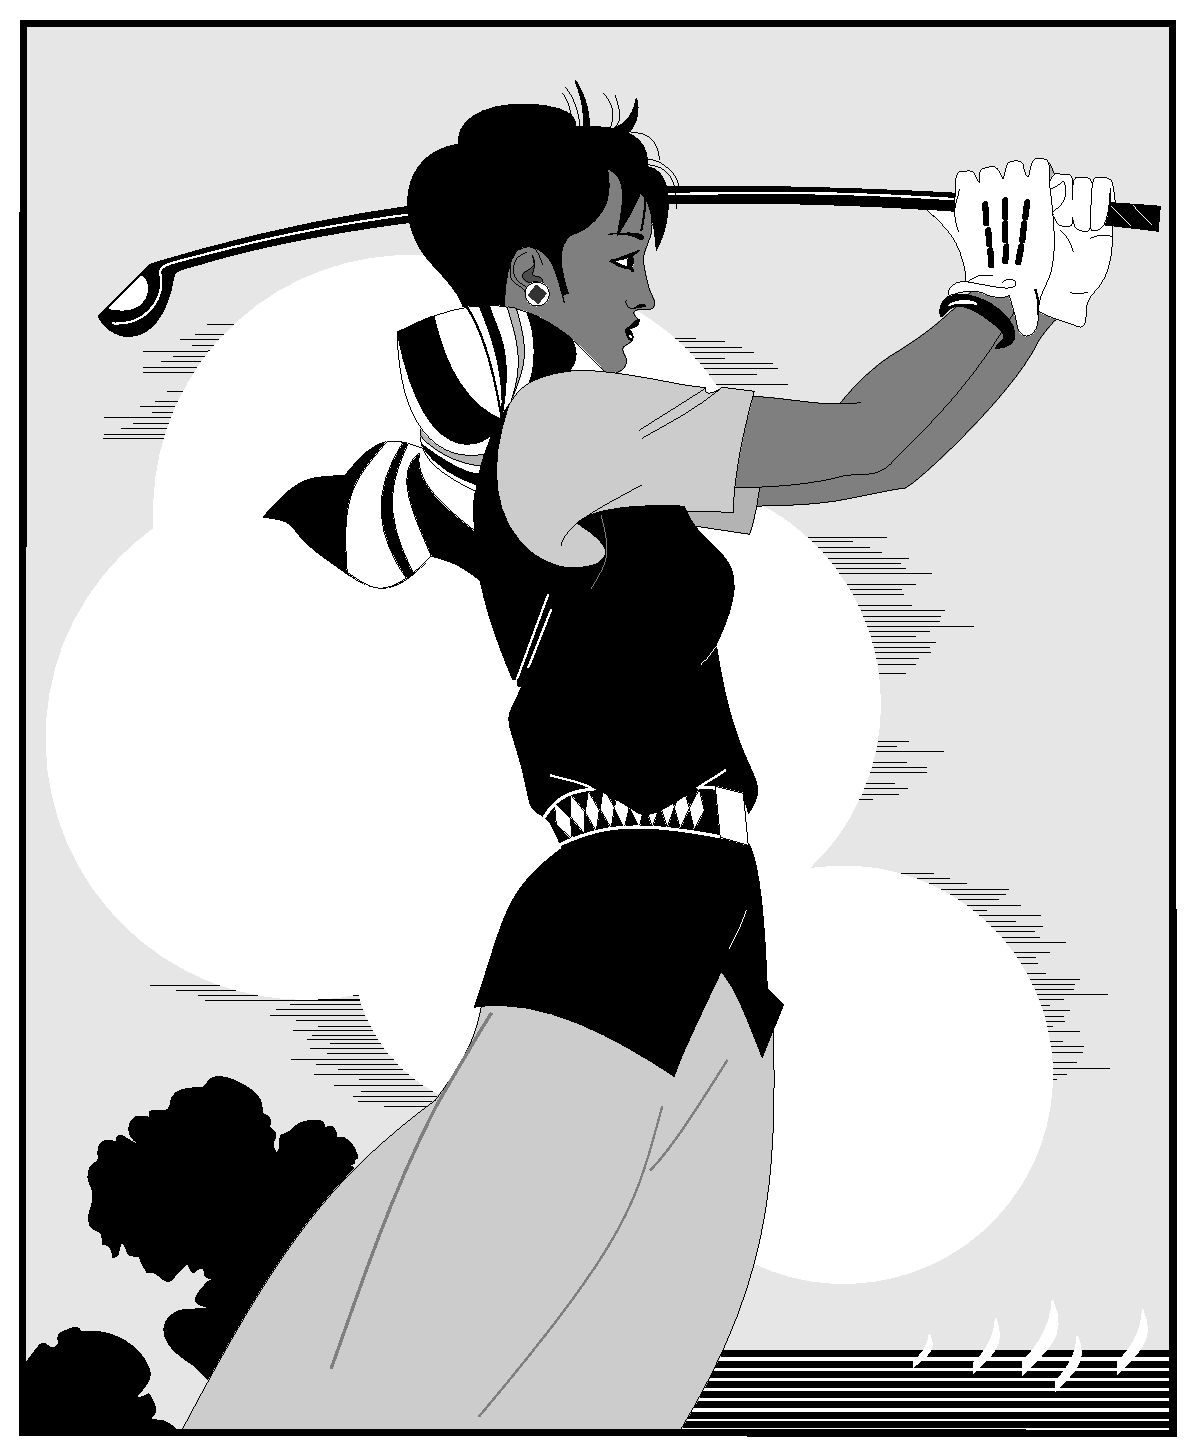
\includegraphics[width=0.2\textwidth]{golfer}}
			\fbox{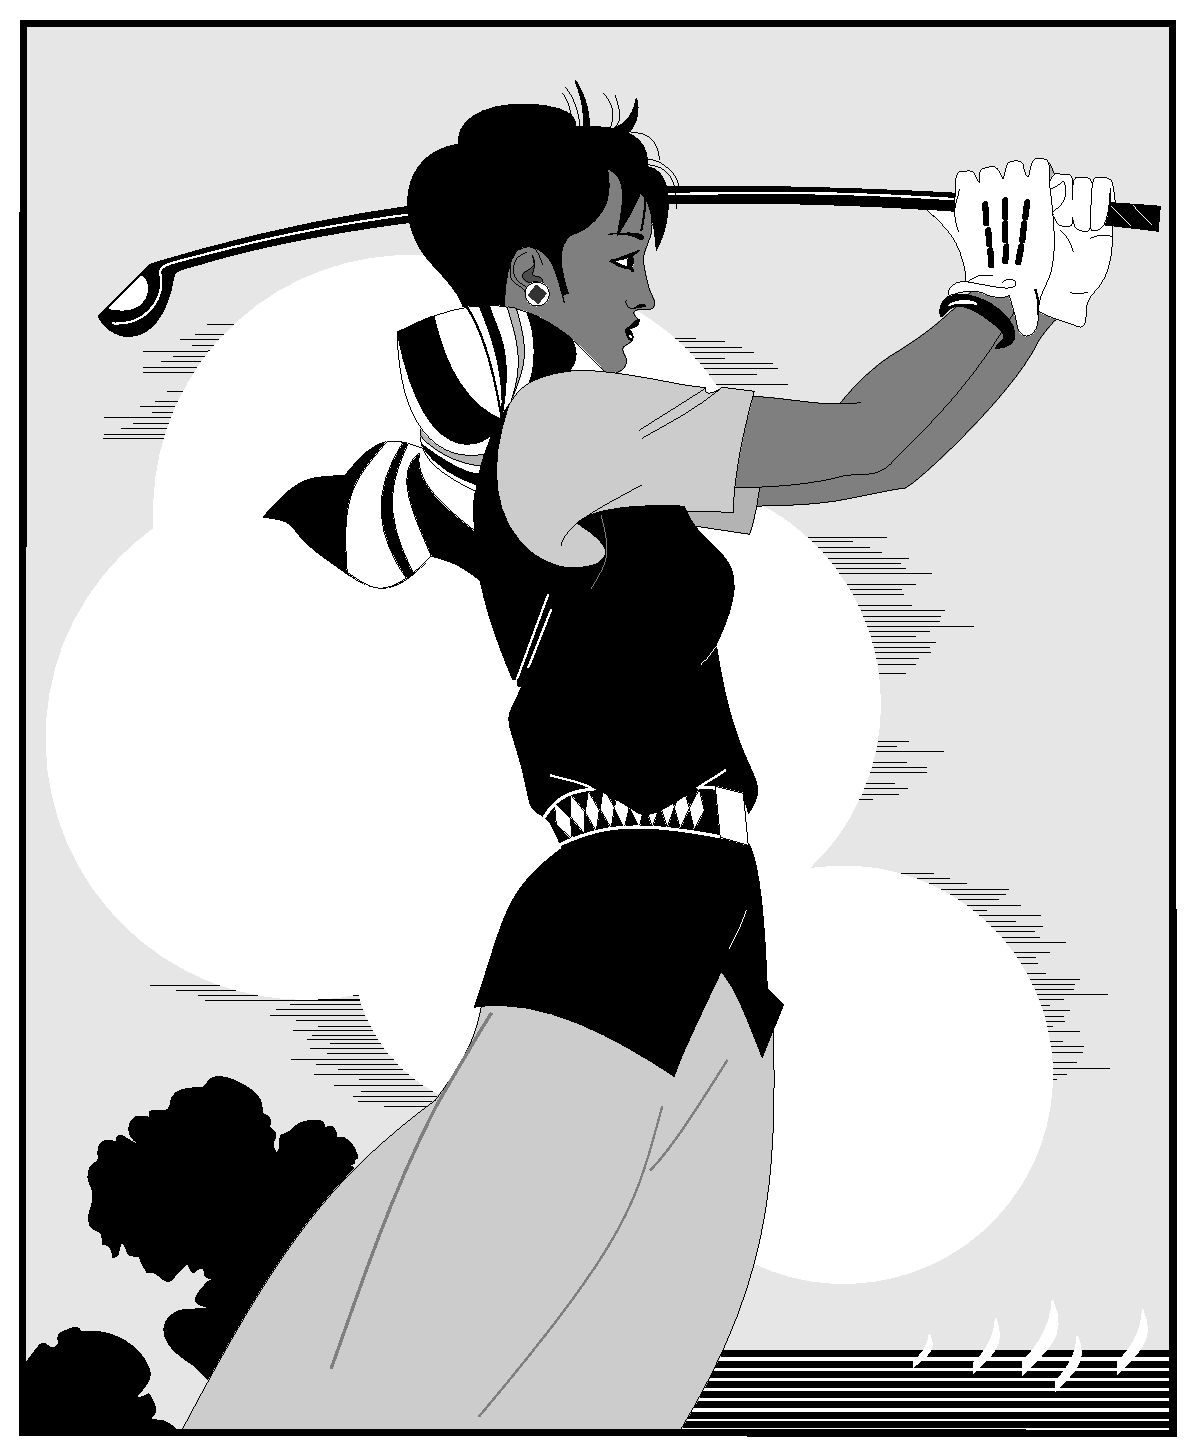
\includegraphics[width=0.2\textwidth]{golfer}}
			\fbox{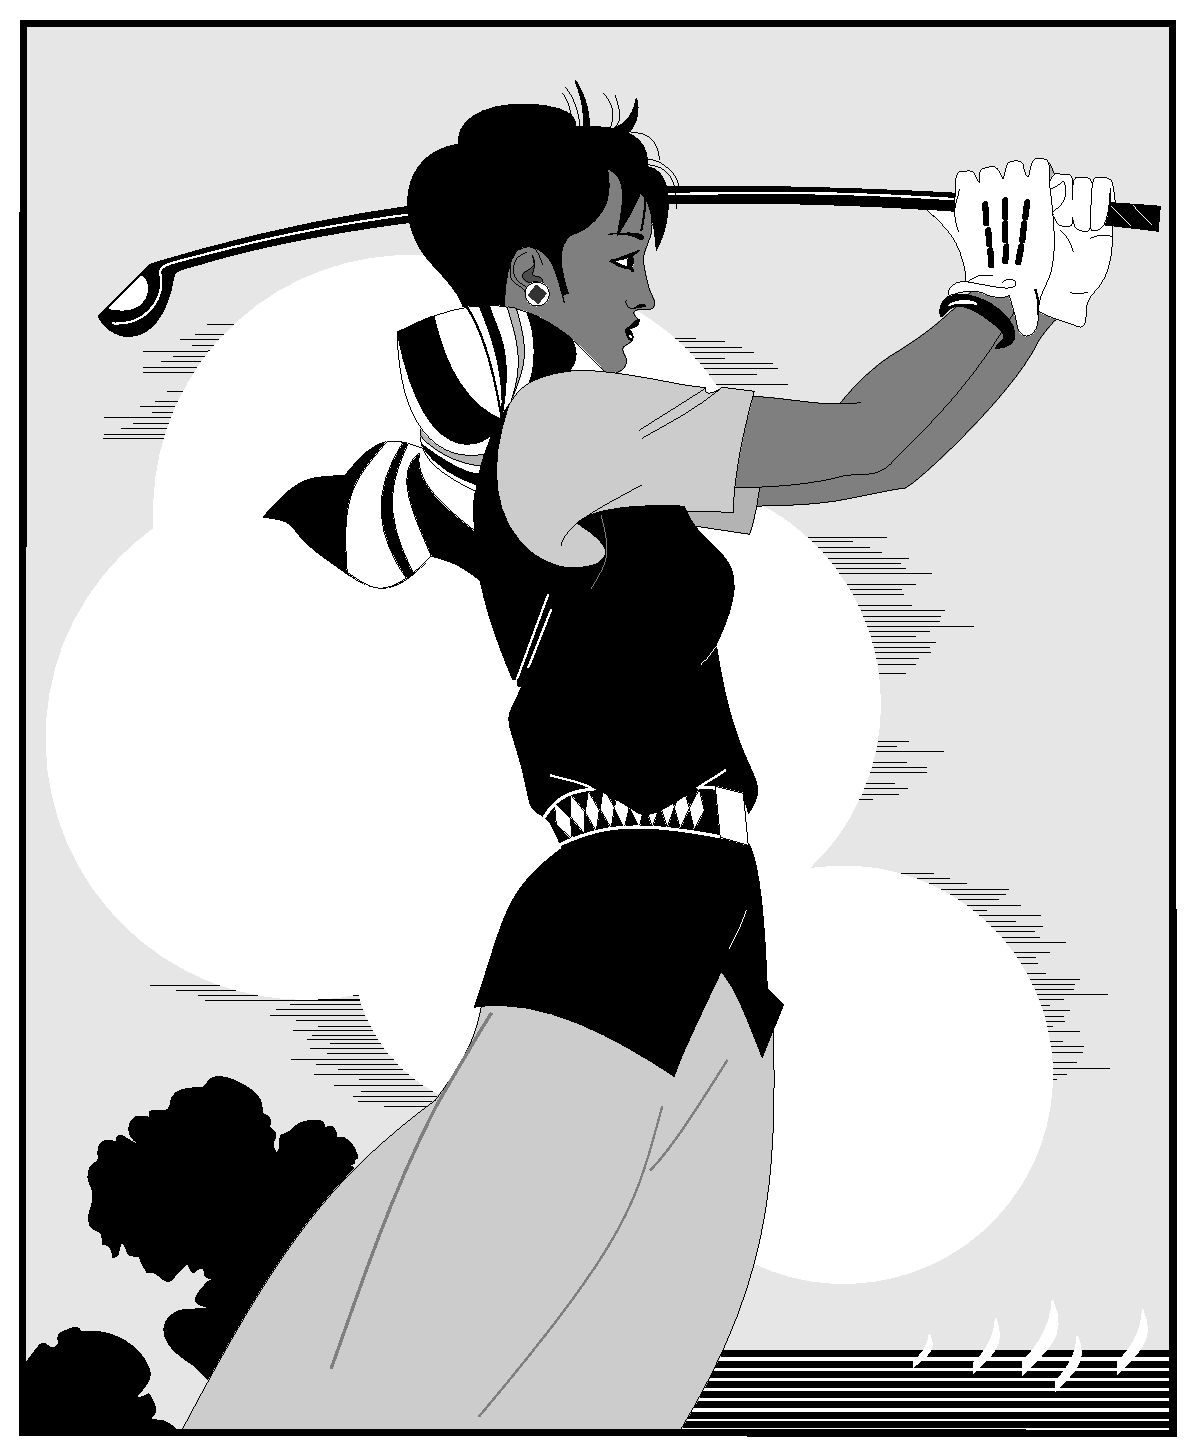
\includegraphics[width=0.2\textwidth]{golfer}}
			\fbox{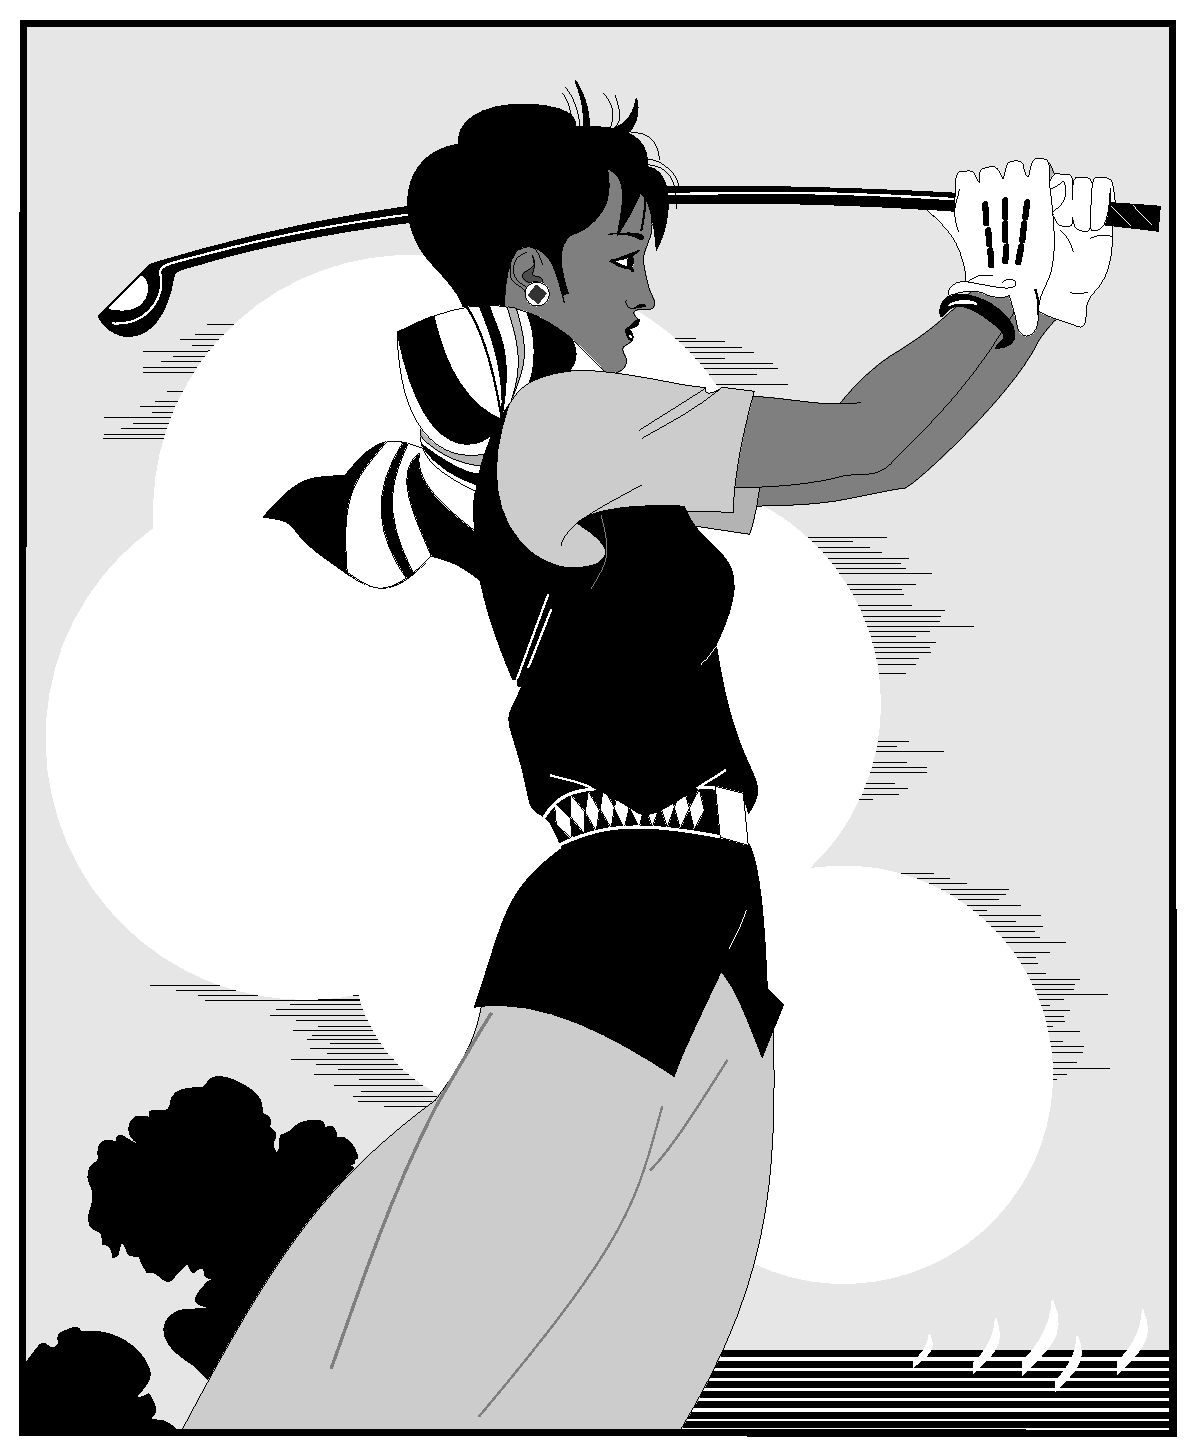
\includegraphics[width=0.2\textwidth]{golfer}}
\bicaption[golfer7]{}{打高尔夫球的人(非规范要求)}{Fig.$\!$}{The person playing golf (Not stated in the regulation)}
		\end{minipage}
	\end{sideways}
\end{figure}

\clearpage

如果不想让图片浮动到下一章节,那么在此处使用\cs{clearpage}命令。

\section{如何做出符合规范的漂亮的图}

关于作图工具在后文\ref{drawtool}中给出一些作图工具的介绍,此处不多言。
此处以R语言和Tikz为例说明如何做出符合规范的图。

\subsection{Tikz作图举例}

使用Tikz作图核心思想是把格式、主题、样式与内容分离,定义在全局中。
注意字体设置可以有两种选择,如何字少,用五号字,字多用小五。
使用Tikz作图不会出现字体问题,字体会自动与正文一致。

\begin{figure}[thb!]
  \centering
      \begin{tikzpicture}[xscale=0.8,yscale=0.3,rotate=90]
        \small
	\draw (-22,6.5) node[refcell]{参考基因组};
	\draw[refline] (-23, 5) -- (27, 5);
	\draw (-22,3.75) node[tscell]{肿瘤样本};
	\draw (-20,3.75) node[tncell]{正常细胞};
	\draw[tnline] (-21, 2.5) -- (27, 2.5);
	\draw (-20,1.25) node[ttcell]{肿瘤细胞};
	\rcell{2}{6};
	\draw[fakeevolve] (4.5, 5.25) -- (4.5, 4.8);
	\ncell{2}{4};
	\draw[evolve] (4.5, 3) .. controls (4.5,2.8) and (-3.5,2.9) ..  (-3.5, 2);
	\draw[evolve] (4.5, 3) .. controls (4.5,2.8) and (11.5,2.9) .. (11.5, 2);
	\tcellone{-6}{1.5};
	\draw (-9, 2) node[ttcell]{1};
	\draw[evolve] (-3.5, 0) .. controls (-3.5,-0.2) and (-12,-0.1) .. (-12, -1.5);
	\draw[evolve] (-3.5, 0) .. controls (-3.5,-0.2) and (1.5,-0.1) .. (1.5, -1.5);
	\tcellthree{7}{1.5};
	\draw (4, 2) node[ttcell]{2};
	\draw[evolve] (11, 0.5) .. controls (11,0.3) and (19,0.4) .. (19, -1.5);
	\tcellfive{-16}{-2};
	\draw (-19, -1.5) node[ttcell]{3};
	\tcelltwo{-1}{-2};
	\draw (-4, -1.5) node[ttcell]{4};
	\tcellfour{12}{-2};
	\draw (9, -1.5) node[ttcell]{5};
      \end{tikzpicture}
  \begin{minipage}{.9\linewidth}
      \vskip 0.2em
      \wuhao 图中,带有箭头的淡蓝色箭头表示肿瘤子种群的进化方向。一般地,从肿瘤组织中取用于进行二代测序的样本中含有一定程度的正常细胞污染,因此肿瘤的样本中含有正常细胞和肿瘤细胞。每一个子种群的基因组的模拟过程是把生殖细胞变异和体细胞变异加入到参考基因组中。
      \vspace{0.6em}
  \end{minipage}
\bicaption[tumor]{}{肿瘤组织中各个子种群的进化示意图}{Fig.$\!$}{The diagram of tumor subpopulation evolution process}
\end{figure}

\subsection{R作图}

R是一种极具有代表性的典型的作图工具,应用广泛。
与Tikz图~\ref{tumor}~不同,R作图分两种情况:(1)可以转换为Tikz码;(2)不可转换为Tikz码。
第一种情况图形简单,图形中不含有很多数据点,使用R语言中的Tikz包即可。
第二种情况是图形复杂,含有海量数据点,这时候不要转成Tikz矢量图,这会使得论文体积巨大。
推荐使用pdf或png非矢量图形。
使用非矢量图形时要注意选择好字号(五号或小五),和字体(宋体、新罗马)然后选择生成图形大小,注意此时在正文中使用\cs{includegraphics}命令导入时,不要像导入矢量图那样控制图形大小,使用图形的原本的
宽度和高度,这样就确保了非矢量图形中的文字与正文一致了。

为了控制\hitszthesis\ 的大小,此处不给出具体举例。

\subsection{专业绘图工具}[Processional drawing tool]
\label{drawtool}

推荐使用tikz包,使用tikz源码绘图的好处是,图片中的字体与正文中的字体一致。具体如
何使用tikz绘图不属于模板范畴。

tikz适合用来画不需要大量实验数据支撑示意图。但R语言等专业绘图工具具有画出各种、
专业、复杂的数据图。R语言中有tikz包,能自动生成tikz码,这样tikz几乎无所不能。
对于排版有极致追求的小伙伴,可以参考
\href{http://www.texample.net/tikz/resources/}{http://www.texample.net/tikz/resources/}
中所列工具,几乎所有作图软件所作的图形都可转成tikz,然后可以自由的在tikz中修改
图中内容,定义字体等等。实现前文窝工规范中要求的图中字体的一致性的终极目标。

\lipsum[1]

\section{本章小结}[Brief summary]

\lipsum[1]


% 第3章
% !TEX root = ../main.tex



% 第4章
% !TEX root = ../main.tex



% 第5章
% !TEX root = ../main.tex

\chapter{引用参考文献}[Cite reference]

\section{引言}[Introduction]

\lipsum[1]

\section{参考文献引用方法}[How to cite the reference]

\sindex[china]{du!段誉}引文标注遵照GB/T7714-2005,采用顺序编码制。正文中引用文献的标示应置于所引内容最后一个字的右上角,所引文献编号用阿拉伯数字置于方括号“[ ]”中,用小4号字体的上角标。要求:

(1)引用单篇文献时,如“二次铣削\cite{ren2010}”。

(2)同一处引用多篇文献时,各篇文献的序号在方括号内全部列出,各序号间用“,”,如
遇连续序号,可标注讫序号。如,…形成了多种数学模型\cite{Gravagne2003,ren2010}…
注意此处添加\cs{inlinecite}中文空格\inlinecite{Gravagne2003,ren2010},可以在cfg文件中修改空格类型。

(3)多次引用同一文献时,在文献序号的“[ ]”后标注引文页码。如,…间质细胞CAMP含量
测定\cite[100-197]{Gravagne2003}…。…含量测定方法规定
\cite[92]{Gravagne2003}…。

(4)当提及的参考文献为文中直接说明时,则用小4号字与正文排齐,如“由文献\inlinecite{webster2010}可知”

(5)多\cite{liu2016}引\cite{fu2018}用\cite{zhai2015}一\cite{yao2015}些\cite{jones2006}参\cite{mcmahan2005}考\cite{jones2004}文献以生成附录参考文献。

\section{本章小结}[Brief summary]

\lipsum[1]


% 第6章
% !TEX root = ../main.tex

% 中英标题:\chapter{中文标题}[英文标题]
\chapter{补充说明}[Complements]

\section{引言}[Introduction]

这是 \hitszthesis\ 的示例文档,基本上覆盖了模板中所有格式的设置。建议大家在使用模
板之前,除了阅读《\hitszthesis\:哈尔滨工业大学学位论文模板》\footnote{即
hitszthesis.pdf文件},本示例文档也最好能看一看。此示例文档尽量使用到所有的排版格式
,然而对于一些不在我工规范中规定的文档,理论上是由用户自由发挥,这里不给出样例
。需要另行载入的宏包和自定义命令在文件`hitszthesis.sty'中有示例,这里不列举。

\section{关于数字}[Number]

按《关于出版物上数字用法的试行规定》(1987年1月1日国家语言文字工作委员会等7个单位公布),除习惯用中文数字表示的以外,一般数字均用阿拉伯数字。
(1)公历的世纪、年代、年、月、日和时刻一律用阿拉伯数字,如20世纪,80年代,4时3刻等。年号要用四位数,如1989年,不能用89年。
(2)记数与计算(含正负整数、分数、小数、百分比、约数等)一律用阿拉伯数字,如3/4,4.5\%,10个月,500多种等。
(3)一个数值的书写形式要照顾到上下文。不是出现在一组表示科学计量和具有统计意义数字中的一位数可以用汉字,如一个人,六条意见。星期几一律用汉字,如星期六。邻近两个数字并列连用,表示概数,应该用汉字数字,数字间不用顿号隔开,如三五天,七八十种,四十五六岁,一千七八百元等。
(4)数字作为词素构成定型的词、词组、惯用语、缩略语等应当使用汉字。如二倍体,三叶虫,第三世界,“七五”规划,相差十万八千里等。
(5)5位以上的数字,尾数零多的,可改写为以万、亿为单位的数。一般情况下不得以十、百、千、十万、百万、千万、十亿、百亿、千亿作为单位。如~\num{345000000}~公里可改写为3.45亿公里或~\num{34500}~万公里,但不能写为3亿~\num{4500}~万公里或3亿4千5百万公里。
(6)数字的书写不必每格一个数码,一般每两数码占一格,数字间分节不用分位号“,”,凡4位或4位以上的数都从个位起每3位数空半个数码(1/4汉字)。“\num{3000000}”,不要写成“3,000,000”,小数点后的数从小数点起向右按每三位一组分节。一个用阿拉伯数字书写的多位数不能从数字中间转行。
(7)数量的增加或减少要注意下列用词的概念:1)增加为(或增加到)过去的二倍,即过去为一,现在为二;2)增加(或增加了)二倍,即过去为一,现在为三;3)超额80\%,即定额为100,现在为180;4)降低到80\%,即过去为100,现在为80;5)降低(或降低了)80\%,即原来为100,现在为20;6)为原数的1/4,即原数为4,现在为1,或原数为1,现在为0.25。
应特别注意在表达数字减小时,不宜用倍数,而应采用分数。如减少为原来的1/2,1/3等。

\section{索引示例}[Index]

为便于检索文中内容,可编制索引置于论文之后(根据需要决定是否设置)。索引以论文中
的专业词语为检索线索,指出其相关内容的所在页码。索引用中、英两种文字书写,中文在
前。\sindex[china]{qi!乔峰}\sindex[english]{Xu Zhu}\sindex[english]{Qiao Feng}
中文按各词汉语拼音第一个字母排序,英文按该词第一个英文字母排序。

\section{术语排版举例}[Glossaries and index]

术语的定义和使用可以结合索引,灵活使用。例如,\gtssbp 是一种应用于狄利克雷过程抽样的算法。下次出现将是另一种格式:\gtssbp 。还可以切换单复数例如:\gscna ,下次出现为:\gscnas 。此处体现了\LaTeX\ 格式内容分离的优势。

\section{定理和定义等}[Theorem]

\begin{theorem}[\cite{ren2010}]
宇宙大爆炸是一种爆炸。
\end{theorem}
\begin{definition}[(霍金)]
宇宙大爆炸是一种爆炸。
\end{definition}
\begin{assumption}
宇宙大爆炸是一种爆炸。
\end{assumption}
\begin{lemma}
宇宙大爆炸是一种爆炸。
\end{lemma}
\begin{corollary}
宇宙大爆炸是一种爆炸。
\end{corollary}
\begin{exercise}
宇宙大爆炸是一种爆炸。
\end{exercise}
\begin{problem}[(Albert Einstein)]
宇宙大爆炸是一种爆炸。
\end{problem}
\begin{remark}
宇宙大爆炸是一种爆炸。
\end{remark}
\begin{axiom}[(爱因斯坦)]
宇宙大爆炸是一种爆炸。
\end{axiom}
\begin{conjecture}
宇宙大爆炸是一种爆炸。
\end{conjecture}

\lipsum[1]

\section{其他杂项}[Miscellaneous]

\subsection{右翻页}[Open right]

对于双面打印的论文,强制使每章的标题页出现右手边为右翻页。规范中没有明确规定是否是右翻页打印。模板给出了右翻页选项。为了应对用户的个人喜好,在希望设置成右翻页的位置之前添加\cs{cleardoublepage}命令即可。

\subsection{算法}[Algorithms]

算法不在规范中要求,在hitszthesis.sty中有相关定义,一个例子如算法\ref{alg:rerank}所示。
\begin{algorithm}
  \DontPrintSemicolon
  \wuhao
  \caption{混合重排算法}
  \label{alg:rerank}
  \KwData{$A$:待重排的元素集合 \newline
  $\alpha$: 对多样性,相关性作折中的权重因子}
  \KwResult{$A_k$: a subset of $A$ of size k}
\end{algorithm}

\subsection{脚注}[Footnotes]

不在再规范\footnote{规范是指\PGR\ 和\UGR}中要求,模板默认使用清华大学的格式。

\subsection{源码}[Source code]

也不在再规范中要求。如果有需要最好使用minted包,但在编译的时候需要添加“-shell-escape”选项且安装pygmentize软件,这些不在模板中默认载入,如果需要自行载入。

\subsection{思源宋体}[Siyuan font]
如果要使用思源字体,需要思源字体的定义文件,此文件请到模板的开发版网址github:
\href{https://gihitb.com/YangLaTeX/hitszthesis}{https://gihitb.com/YangLaTeX/hitszthesis}
处下载。

\subsection{术语词汇管理}[Manage glossaries]

推荐使用glossaries包管理术语、缩略语,可以自动生成首次全写,非首次缩写。

\section{本章小结}[Brief summary]

\lipsum[2]


% 开始写正文之后的部分
\backmatter

%%%% \begin{本科书序} %%%% 这是一个假的环境,本科请用这里的内容

% % 结论
% % !TEX root = ../main.tex

% 结论
\begin{conclusions}

学位论文的结论作为论文正文的最后一章单独排写,但不加章标题序号。

结论应是作者在学位论文研究过程中所取得的创新性成果的概要总结,不能与摘要混为一谈。博士学位论文结论应包括论文的主要结果、创新点、展望三部分,在结论中应概括论文的核心观点,明确、客观地指出本研究内容的创新性成果(含新见解、新观点、方法创新、技术创新、理论创新),并指出今后进一步在本研究方向进行研究工作的展望与设想。对所取得的创新性成果应注意从定性和定量两方面给出科学、准确的评价,分(1)、(2)、(3)…条列出,宜用“提出了”、“建立了”等词叙述。

\end{conclusions}


% % 参考文献
% \bibliographystyle{hitszthesis}
% \bibliography{reference}

% % 授权
% \authorization

% % 授权页为扫描的PDF文件(scan.pdf),与上面的命令互斥
% % \authorization[scan.pdf]

% % 致谢
% % !TEX root = ../main.tex

% 致谢
\begin{acknowledgements}
衷心感谢导师~XXX~教授对本人的精心指导。他的言传身教将使我终生受益。

……

感谢哈深\LaTeX{}论文模板\hitszthesis\ !

\end{acknowledgements}


% % 附录
% \begin{appendix}
%   % !TEX root = ../main.tex

% 附录1
\chapter{外文资料的调研阅读报告或书面翻译}

\title{英文资料的中文标题}

{\heiti 摘要:} 本章为外文资料翻译内容。如果有摘要可以直接写上来,这部分好像没有
明确的规定。

\section{单目标规划}
北冥有鱼,其名为鲲。鲲之大,不知其几千里也。化而为鸟,其名为鹏。鹏之背,不知其几
千里也。怒而飞,其翼若垂天之云。是鸟也,海运则将徙于南冥。南冥者,天池也。
\begin{equation}\tag*{(123)}
 p(y|\mathbf{x}) = \frac{p(\mathbf{x},y)}{p(\mathbf{x})}=
\frac{p(\mathbf{x}|y)p(y)}{p(\mathbf{x})}
\end{equation}

吾生也有涯,而知也无涯。以有涯随无涯,殆已!已而为知者,殆而已矣!为善无近名,为
恶无近刑,缘督以为经,可以保身,可以全生,可以养亲,可以尽年。

\subsection{线性规划}
庖丁为文惠君解牛,手之所触,肩之所倚,足之所履,膝之所倚,砉然响然,奏刀騞然,莫
不中音,合于桑林之舞,乃中经首之会。
\begin{table}[ht]
\centering
  \centering
  \caption*{表~1\hskip1em 这是手动编号但不出现在索引中的一个表格例子}
  \label{tab:badtabular3}
  \begin{tabular}[c]{|m{1.5cm}|c|c|c|c|c|c|}\hline
    \multicolumn{2}{|c|}{Network Topology} & \# of nodes &
    \multicolumn{3}{c|}{\# of clients} & Server \\\hline
    GT-ITM & Waxman Transit-Stub & 600 &
    \multirow{2}{2em}{2\%}&
    \multirow{2}{2em}{10\%}&
    \multirow{2}{2em}{50\%}&
    \multirow{2}{1.2in}{Max. Connectivity}\\\cline{1-3}
    \multicolumn{2}{|c|}{Inet-2.1} & 6000 & & & &\\\hline
    & \multicolumn{2}{c|}{ABCDEF} &\multicolumn{4}{c|}{} \\\hline
\end{tabular}
\end{table}

文惠君曰:“嘻,善哉!技盖至此乎?”庖丁释刀对曰:“臣之所好者道也,进乎技矣。始臣之
解牛之时,所见无非全牛者;三年之后,未尝见全牛也;方今之时,臣以神遇而不以目视,
官知止而神欲行。依乎天理,批大郤,导大窾,因其固然。技经肯綮之未尝,而况大坬乎!
良庖岁更刀,割也;族庖月更刀,折也;今臣之刀十九年矣,所解数千牛矣,而刀刃若新发
于硎。彼节者有间而刀刃者无厚,以无厚入有间,恢恢乎其于游刃必有余地矣。是以十九年
而刀刃若新发于硎。虽然,每至于族,吾见其难为,怵然为戒,视为止,行为迟,动刀甚微,
謋然已解,如土委地。提刀而立,为之而四顾,为之踌躇满志,善刀而藏之。”

文惠君曰:“善哉!吾闻庖丁之言,得养生焉。”


\subsection{非线性规划}
孔子与柳下季为友,柳下季之弟名曰盗跖。盗跖从卒九千人,横行天下,侵暴诸侯。穴室枢
户,驱人牛马,取人妇女。贪得忘亲,不顾父母兄弟,不祭先祖。所过之邑,大国守城,小
国入保,万民苦之。孔子谓柳下季曰:“夫为人父者,必能诏其子;为人兄者,必能教其弟。
若父不能诏其子,兄不能教其弟,则无贵父子兄弟之亲矣。今先生,世之才士也,弟为盗
跖,为天下害,而弗能教也,丘窃为先生羞之。丘请为先生往说之。”

柳下季曰:“先生言为人父者必能诏其子,为人兄者必能教其弟,若子不听父之诏,弟不受
兄之教,虽今先生之辩,将奈之何哉?且跖之为人也,心如涌泉,意如飘风,强足以距敌,
辩足以饰非。顺其心则喜,逆其心则怒,易辱人以言。先生必无往。”

孔子不听,颜回为驭,子贡为右,往见盗跖。

\subsection{整数规划}
盗跖乃方休卒徒大山之阳,脍人肝而餔之。孔子下车而前,见谒者曰:“鲁人孔丘,闻将军
高义,敬再拜谒者。”谒者入通。盗跖闻之大怒,目如明星,发上指冠,曰:“此夫鲁国之
巧伪人孔丘非邪?为我告之:尔作言造语,妄称文、武,冠枝木之冠,带死牛之胁,多辞缪
说,不耕而食,不织而衣,摇唇鼓舌,擅生是非,以迷天下之主,使天下学士不反其本,妄
作孝弟,而侥幸于封侯富贵者也。子之罪大极重,疾走归!不然,我将以子肝益昼餔之膳。”
%   % !TEX root = ../main.tex

% 附录2
\chapter{外文资料的调研阅读报告或书面翻译}

\title{英文资料的中文标题}

{\heiti 摘要:} 本章为外文资料翻译内容。如果有摘要可以直接写上来,这部分好像没有
明确的规定。

\section{单目标规划}
北冥有鱼,其名为鲲。鲲之大,不知其几千里也。化而为鸟,其名为鹏。鹏之背,不知其几
千里也。怒而飞,其翼若垂天之云。是鸟也,海运则将徙于南冥。南冥者,天池也。
\begin{equation}\tag*{(123)}
 p(y|\mathbf{x}) = \frac{p(\mathbf{x},y)}{p(\mathbf{x})}=
\frac{p(\mathbf{x}|y)p(y)}{p(\mathbf{x})}
\end{equation}

吾生也有涯,而知也无涯。以有涯随无涯,殆已!已而为知者,殆而已矣!为善无近名,为
恶无近刑,缘督以为经,可以保身,可以全生,可以养亲,可以尽年。

\subsection{线性规划}
庖丁为文惠君解牛,手之所触,肩之所倚,足之所履,膝之所倚,砉然响然,奏刀騞然,莫
不中音,合于桑林之舞,乃中经首之会。
\begin{table}[ht]
\centering
  \centering
  \caption*{表~1\hskip1em 这是手动编号但不出现在索引中的一个表格例子}
  \label{tab:badtabular3}
  \begin{tabular}[c]{|m{1.5cm}|c|c|c|c|c|c|}\hline
    \multicolumn{2}{|c|}{Network Topology} & \# of nodes &
    \multicolumn{3}{c|}{\# of clients} & Server \\\hline
    GT-ITM & Waxman Transit-Stub & 600 &
    \multirow{2}{2em}{2\%}&
    \multirow{2}{2em}{10\%}&
    \multirow{2}{2em}{50\%}&
    \multirow{2}{1.2in}{Max. Connectivity}\\\cline{1-3}
    \multicolumn{2}{|c|}{Inet-2.1} & 6000 & & & &\\\hline
    & \multicolumn{2}{c|}{ABCDEF} &\multicolumn{4}{c|}{} \\\hline
\end{tabular}
\end{table}

文惠君曰:“嘻,善哉!技盖至此乎?”庖丁释刀对曰:“臣之所好者道也,进乎技矣。始臣之
解牛之时,所见无非全牛者;三年之后,未尝见全牛也;方今之时,臣以神遇而不以目视,
官知止而神欲行。依乎天理,批大郤,导大窾,因其固然。技经肯綮之未尝,而况大坬乎!
良庖岁更刀,割也;族庖月更刀,折也;今臣之刀十九年矣,所解数千牛矣,而刀刃若新发
于硎。彼节者有间而刀刃者无厚,以无厚入有间,恢恢乎其于游刃必有余地矣。是以十九年
而刀刃若新发于硎。虽然,每至于族,吾见其难为,怵然为戒,视为止,行为迟,动刀甚微,
謋然已解,如土委地。提刀而立,为之而四顾,为之踌躇满志,善刀而藏之。”

文惠君曰:“善哉!吾闻庖丁之言,得养生焉。”


\subsection{非线性规划}
孔子与柳下季为友,柳下季之弟名曰盗跖。盗跖从卒九千人,横行天下,侵暴诸侯。穴室枢
户,驱人牛马,取人妇女。贪得忘亲,不顾父母兄弟,不祭先祖。所过之邑,大国守城,小
国入保,万民苦之。孔子谓柳下季曰:“夫为人父者,必能诏其子;为人兄者,必能教其弟。
若父不能诏其子,兄不能教其弟,则无贵父子兄弟之亲矣。今先生,世之才士也,弟为盗
跖,为天下害,而弗能教也,丘窃为先生羞之。丘请为先生往说之。”

柳下季曰:“先生言为人父者必能诏其子,为人兄者必能教其弟,若子不听父之诏,弟不受
兄之教,虽今先生之辩,将奈之何哉?且跖之为人也,心如涌泉,意如飘风,强足以距敌,
辩足以饰非。顺其心则喜,逆其心则怒,易辱人以言。先生必无往。”

孔子不听,颜回为驭,子贡为右,往见盗跖。

\subsection{整数规划}
盗跖乃方休卒徒大山之阳,脍人肝而餔之。孔子下车而前,见谒者曰:“鲁人孔丘,闻将军
高义,敬再拜谒者。”谒者入通。盗跖闻之大怒,目如明星,发上指冠,曰:“此夫鲁国之
巧伪人孔丘非邪?为我告之:尔作言造语,妄称文、武,冠枝木之冠,带死牛之胁,多辞缪
说,不耕而食,不织而衣,摇唇鼓舌,擅生是非,以迷天下之主,使天下学士不反其本,妄
作孝弟,而侥幸于封侯富贵者也。子之罪大极重,疾走归!不然,我将以子肝益昼餔之膳。”

%   % !TEX root = ../main.tex

% 附录3
\chapter{其它附录}

其他的附录如数据、代码等,可以放在这里。

% \end{appendix}

%%%% \end{本科书序}


%%%% \begin{硕博书序} %%%% 这是一个假的环境,硕、博请用这里的内容

% 结论
% !TEX root = ../main.tex

% 结论
\begin{conclusions}

学位论文的结论作为论文正文的最后一章单独排写,但不加章标题序号。

结论应是作者在学位论文研究过程中所取得的创新性成果的概要总结,不能与摘要混为一谈。博士学位论文结论应包括论文的主要结果、创新点、展望三部分,在结论中应概括论文的核心观点,明确、客观地指出本研究内容的创新性成果(含新见解、新观点、方法创新、技术创新、理论创新),并指出今后进一步在本研究方向进行研究工作的展望与设想。对所取得的创新性成果应注意从定性和定量两方面给出科学、准确的评价,分(1)、(2)、(3)…条列出,宜用“提出了”、“建立了”等词叙述。

\end{conclusions}


% 参考文献
\bibliographystyle{hitszthesis}
\bibliography{reference}

% 附录
\begin{appendix}
  % !TEX root = ../main.tex

% 附录A
\chapter{带章节的附录}[Full Appendix]%
完整的附录内容,包含章节,公式,图表等

\section{附录节的内容}[Section in Appendix]
这是附录的节的内容

附录中图的示例:
\begin{figure}[htbp]
\centering
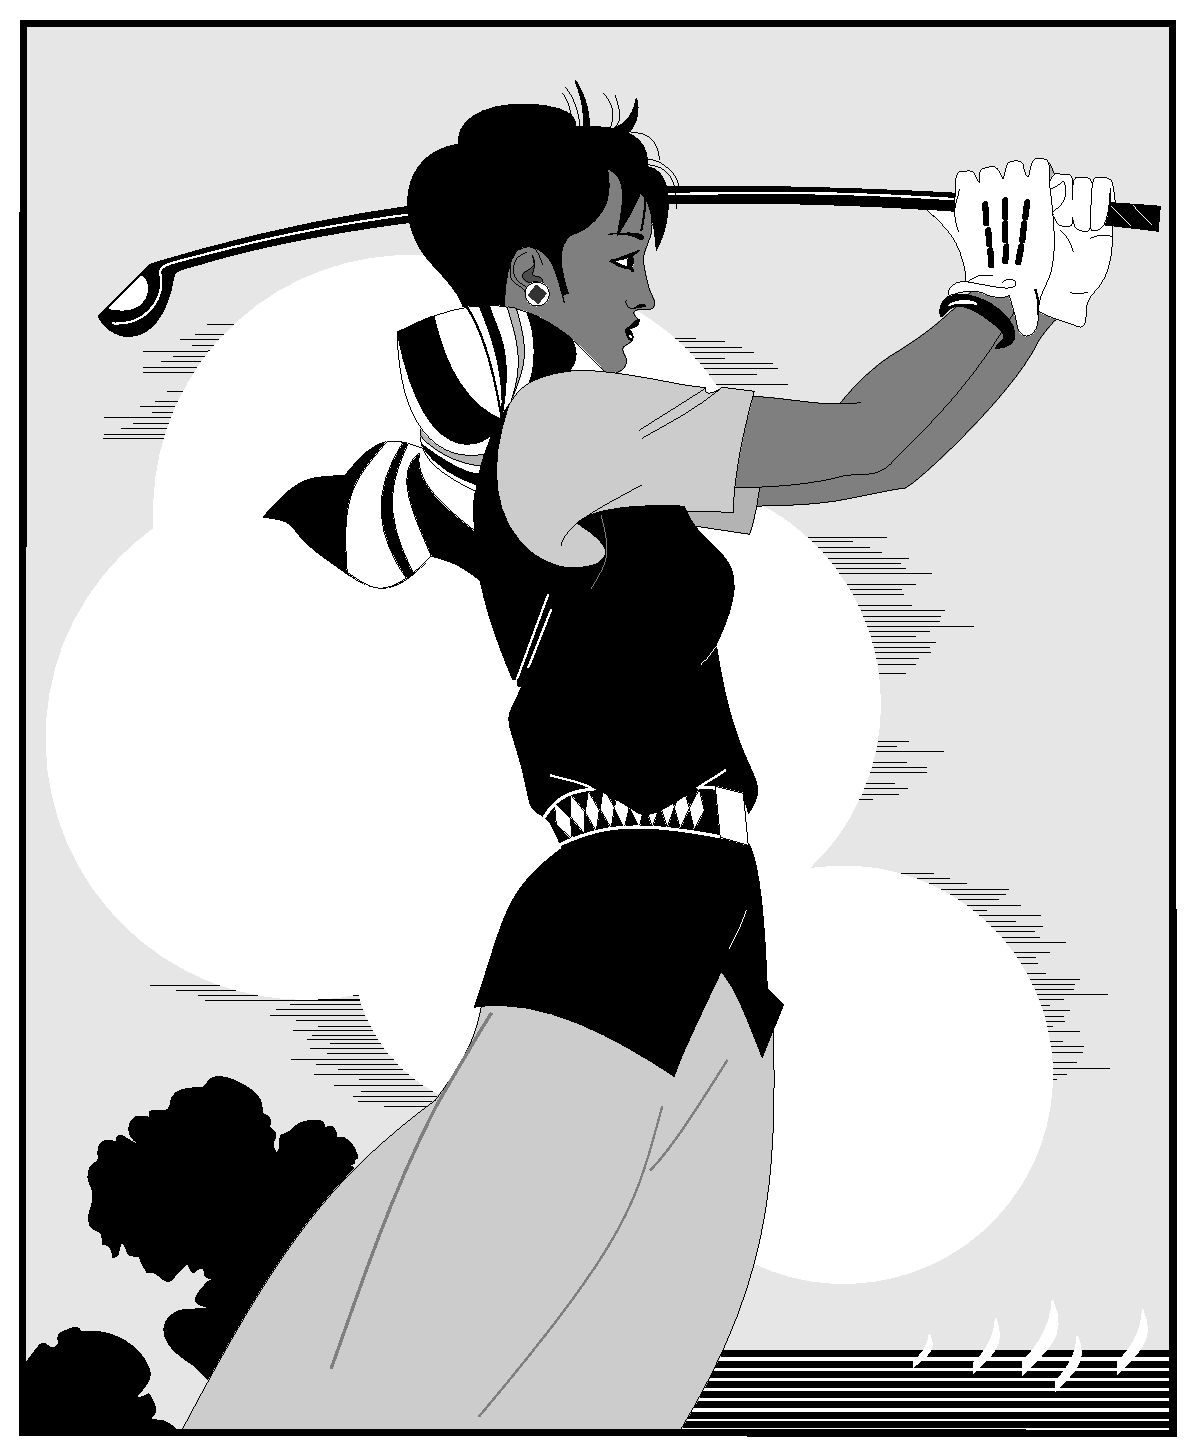
\includegraphics[width = 0.4\textwidth]{golfer}
%\bicaption[golfer5]{}{\xiaosi[0]打高尔夫球的人}{Fig.$\!$}{The person playing golf}\vspace{-1em}
\caption{\xiaosi[0]打高尔夫球的人}
\end{figure}

附录中公式的示例:
\begin{align}
a & = b \times c \\
E & = m c^2
\label{eq}
\end{align}

  % !TEX root = ../main.tex

% 附录B
\chapter{这个星球上最好的免费Linux软件列表}[List of the Best Linux Software in our Planet]
\section{系统}

\href{http://fvwm.org/}{FVWM 自从上世纪诞生以来,此星球最强大的窗口管理器。}
推荐基于FVWM的桌面设计hifvwm:\href{https://github.com/dustincys/hifvwm}{https://github.com/dustincys/hifvwm}。

\subsection{hifvwm的优点}

\begin{enumerate}
	\item 即使打开上百个窗口也不会“蒙圈”。计算机性能越来越强大,窗口任务的管理必须要升级到打怪兽级别。
	\item 自动同步Bing搜索主页的壁纸。每次电脑开机,午夜零点自动更新,用户
		也可以手动更新,从此审美再也不疲劳。
	\item 切换窗口自动聚焦到最上面的窗口。使用键盘快捷键切换窗口时候,减少
		操作过程,自动聚焦到目标窗口。这一特性是虚拟窗口必须的人性化设
		计。
	\item 类似window右下角的功能的最小化窗口来显示桌面的功能此处类似
		win7/win10,实现在一个桌面之内操作多个任务。
	\item 任务栏结合标题栏。采用任务栏和标题栏结合,节省空间。
	\item 同类窗口切换。可以在同类窗口之内类似alt-tab的方式切换。
	\item ……
\end{enumerate}

\section{其他}

\href{https://orgmode.org/}{orgmode,最强大的笔记系统,从来没有之一。}

\href{https://www.jianguoyun.com/}{坚果云,国内一款支持WebDav的云盘系统,国内真正的云盘没有之一。}

\section{vim}
实现中英文每一句一行,以及实现每一句折叠断行的简单正则式,tex源码更加乖乖。
\begin{lstlisting}
vnoremap <leader>fae J:s/[.!?]\zs\s\+/\="\r".matchstr(getline('.'), '^\s*')/g<CR>
vnoremap <leader>fac J:s/[。!?]/\=submatch(0)."\n".matchstr(getline('.'), '^\s*')/g<CR>
vnoremap <leader>fle :!fmt -80 -s<CR>
\end{lstlisting}

\end{appendix}

% 发表文章
% !TEX root = ../main.tex

% 发表论文、专利、获奖情况
\begin{publication}
  \noindent\textbf{(一)发表的学术论文}
  \begin{publist}
    \item	XXX,XXX. Static Oxidation Model of Al-Mg/C Dissipation Thermal Protection Materials[J]. Rare Metal Materials and Engineering, 2010, 39(Suppl. 1): 520-524.(SCI~收录,IDS号为~669JS,IF=0.16)
    \item XXX,XXX. 精密超声振动切削单晶铜的计算机仿真研究[J]. 系统仿真学报,2007,19(4):738-741,753.(EI~收录号:20071310514841)
    \item XXX,XXX. 局部多孔质气体静压轴向轴承静态特性的数值求解[J]. 摩擦学学报,2007(1):68-72.(EI~收录号:20071510544816)
    \item XXX,XXX. 硬脆光学晶体材料超精密切削理论研究综述[J]. 机械工程学报,2003,39(8):15-22.(EI~收录号:2004088028875)
    \item XXX,XXX. 基于遗传算法的超精密切削加工表面粗糙度预测模型的参数辨识以及切削参数优化[J]. 机械工程学报,2005,41(11):158-162.(EI~收录号:2006039650087)
    \item XXX,XXX. Discrete Sliding Mode Cintrok with Fuzzy Adaptive Reaching Law on 6-PEES Parallel Robot[C]. Intelligent System Design and Applications, Jinan, 2006: 649-652.(EI~收录号:20073210746529)
  \end{publist}

  \noindent\textbf{(二)申请及已获得的专利(无专利时此项不必列出)}
  \begin{publist}
    \item XXX,XXX. 一种温热外敷药制备方案:中国,88105607.3[P]. 1989-07-26.
  \end{publist}

  \noindent\textbf{(三)参与的科研项目及获奖情况}
  \begin{publist}
    \item	XXX,XXX. XX~气体静压轴承技术研究, XX~省自然科学基金项目.课题编号:XXXX.
    \item XXX,XXX. XX~静载下预应力混凝土房屋结构设计统一理论. 黑江省科学技术二等奖, 2007.
  \end{publist}
  %\vfill
  %\hangafter=1\hangindent=2em\noindent
  %\setlength{\parindent}{2em}
\end{publication}


% 索引
% % !TEX root = ../main.tex

% 中英文索引
\begin{ceindex}
  \printsubindex*
\end{ceindex}


% 授权
\authorization

% 授权页为扫描的PDF文件(scan.pdf),与上面的命令互斥
% \authorization[scan.pdf]

% 致谢
% !TEX root = ../main.tex

% 致谢
\begin{acknowledgements}
衷心感谢导师~XXX~教授对本人的精心指导。他的言传身教将使我终生受益。

……

感谢哈深\LaTeX{}论文模板\hitszthesis\ !

\end{acknowledgements}


% 个人简介
% !TEX root = ../main.tex

% 个人简历
\begin{resume}

  XXXX~年~XX~月~XX~日出生于~XXXX。

  XXXX~年~XX~月考入~XX~大学~XX~院(系)XX~专业,XXXX~年~XX~月本科毕业并获得~XX~学学士学位。

  XXXX~年~XX~月------XXXX~年~XX~月在~XX~大学~XX~院(系)XX~学科学习并获得~XX~学硕士学位。

  XXXX~年~XX~月------XXXX~年~XX~月在~XX~大学~XX~院(系)XX~学科学习并获得~XX~学博士学位。

  获奖情况:如获三好学生、优秀团干部、X~奖学金等(不含科研学术获奖)。

  工作经历:

  \songti\textbf{(除全日制硕士生以外,其余学生均应增列此项。个人简历一般应包含教育经历和工作经历。)}

\end{resume}


%%%% \end{硕博书序}


% 结束文档撰写
\end{document}
%%=============================================

% Local Variables:
% TeX-engine: xetex
% End:
